\documentclass[aspectratio=169]{beamer}
\usetheme{blob}
\usepackage[normalem]{ulem}

\title{Hopping on the Margins}
\subtitle{with Yifan Wang, and Quinten Weller}
\author{Panos Oikonomou}
\institute{New York University}
\date{\today}

\begin{document}

% ════════════════════════════════════════════════════════════════
% Set up the title slide with a custom background
{
  \setbeamertemplate{background}{\begin{tikzpicture}[remember picture, overlay]
  \node[anchor=north east,xshift=-0.065\paperwidth, yshift=-0.3\paperheight] at (current page.north east) {%
    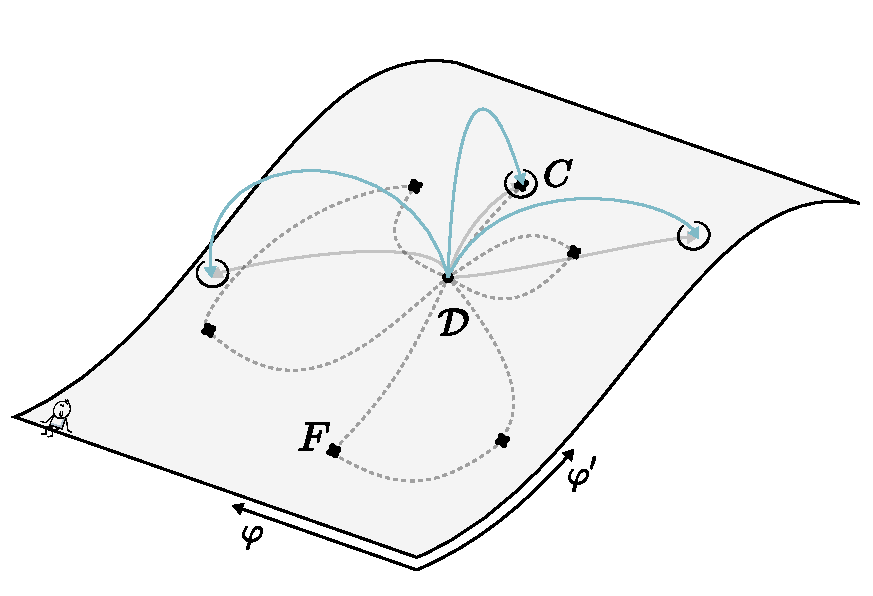
\includegraphics[width=0.5\linewidth]{media/hopping-margin.pdf}
  };
\end{tikzpicture}%
} 
  \begin{frame}[plain]
    \titlepage
  \end{frame}
}
% ════════════════════════════════════════════════════════════════


\section{Motivation}
\begin{frame}
  \frametitle{Defects in the wild}
  \framesubtitle{Using spin chains to pull out conformal defects}
  \begin{figure}
    \centering
    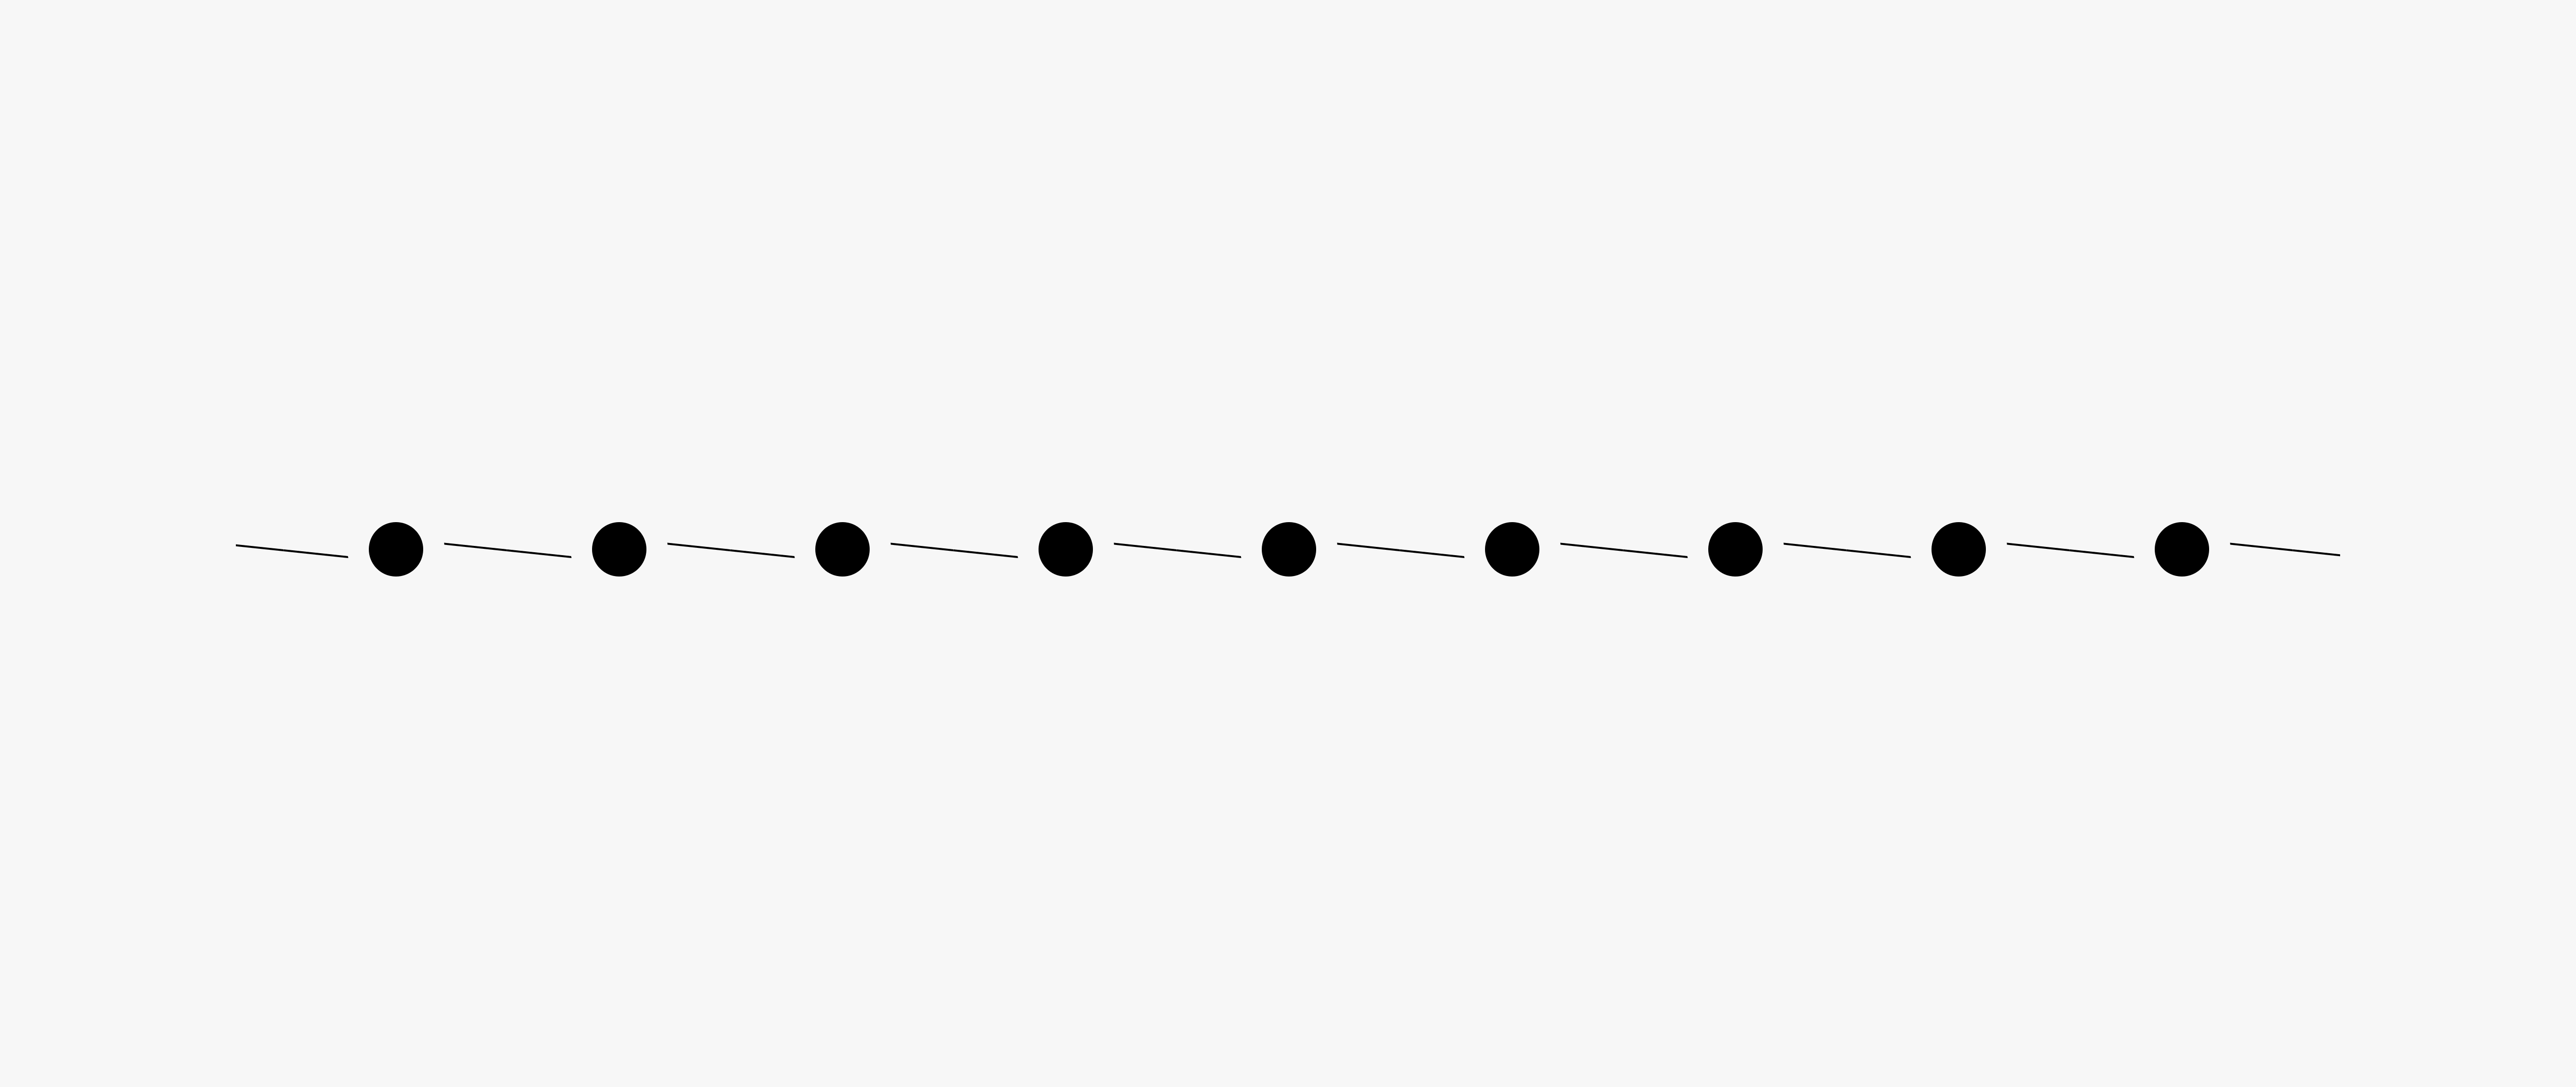
\includegraphics[width=0.8\linewidth]{media/lattice.png}
  \end{figure}
  \begin{equation*}
      H = -J\sum_{n} x_nx_{n+1} - h\sum_{n} z_n
  \end{equation*}
\end{frame}

\begin{frame}
  \frametitle{Defects in the wild}
  \framesubtitle{Using spin chains to pull out conformal defects}
  \begin{figure}
    \centering
    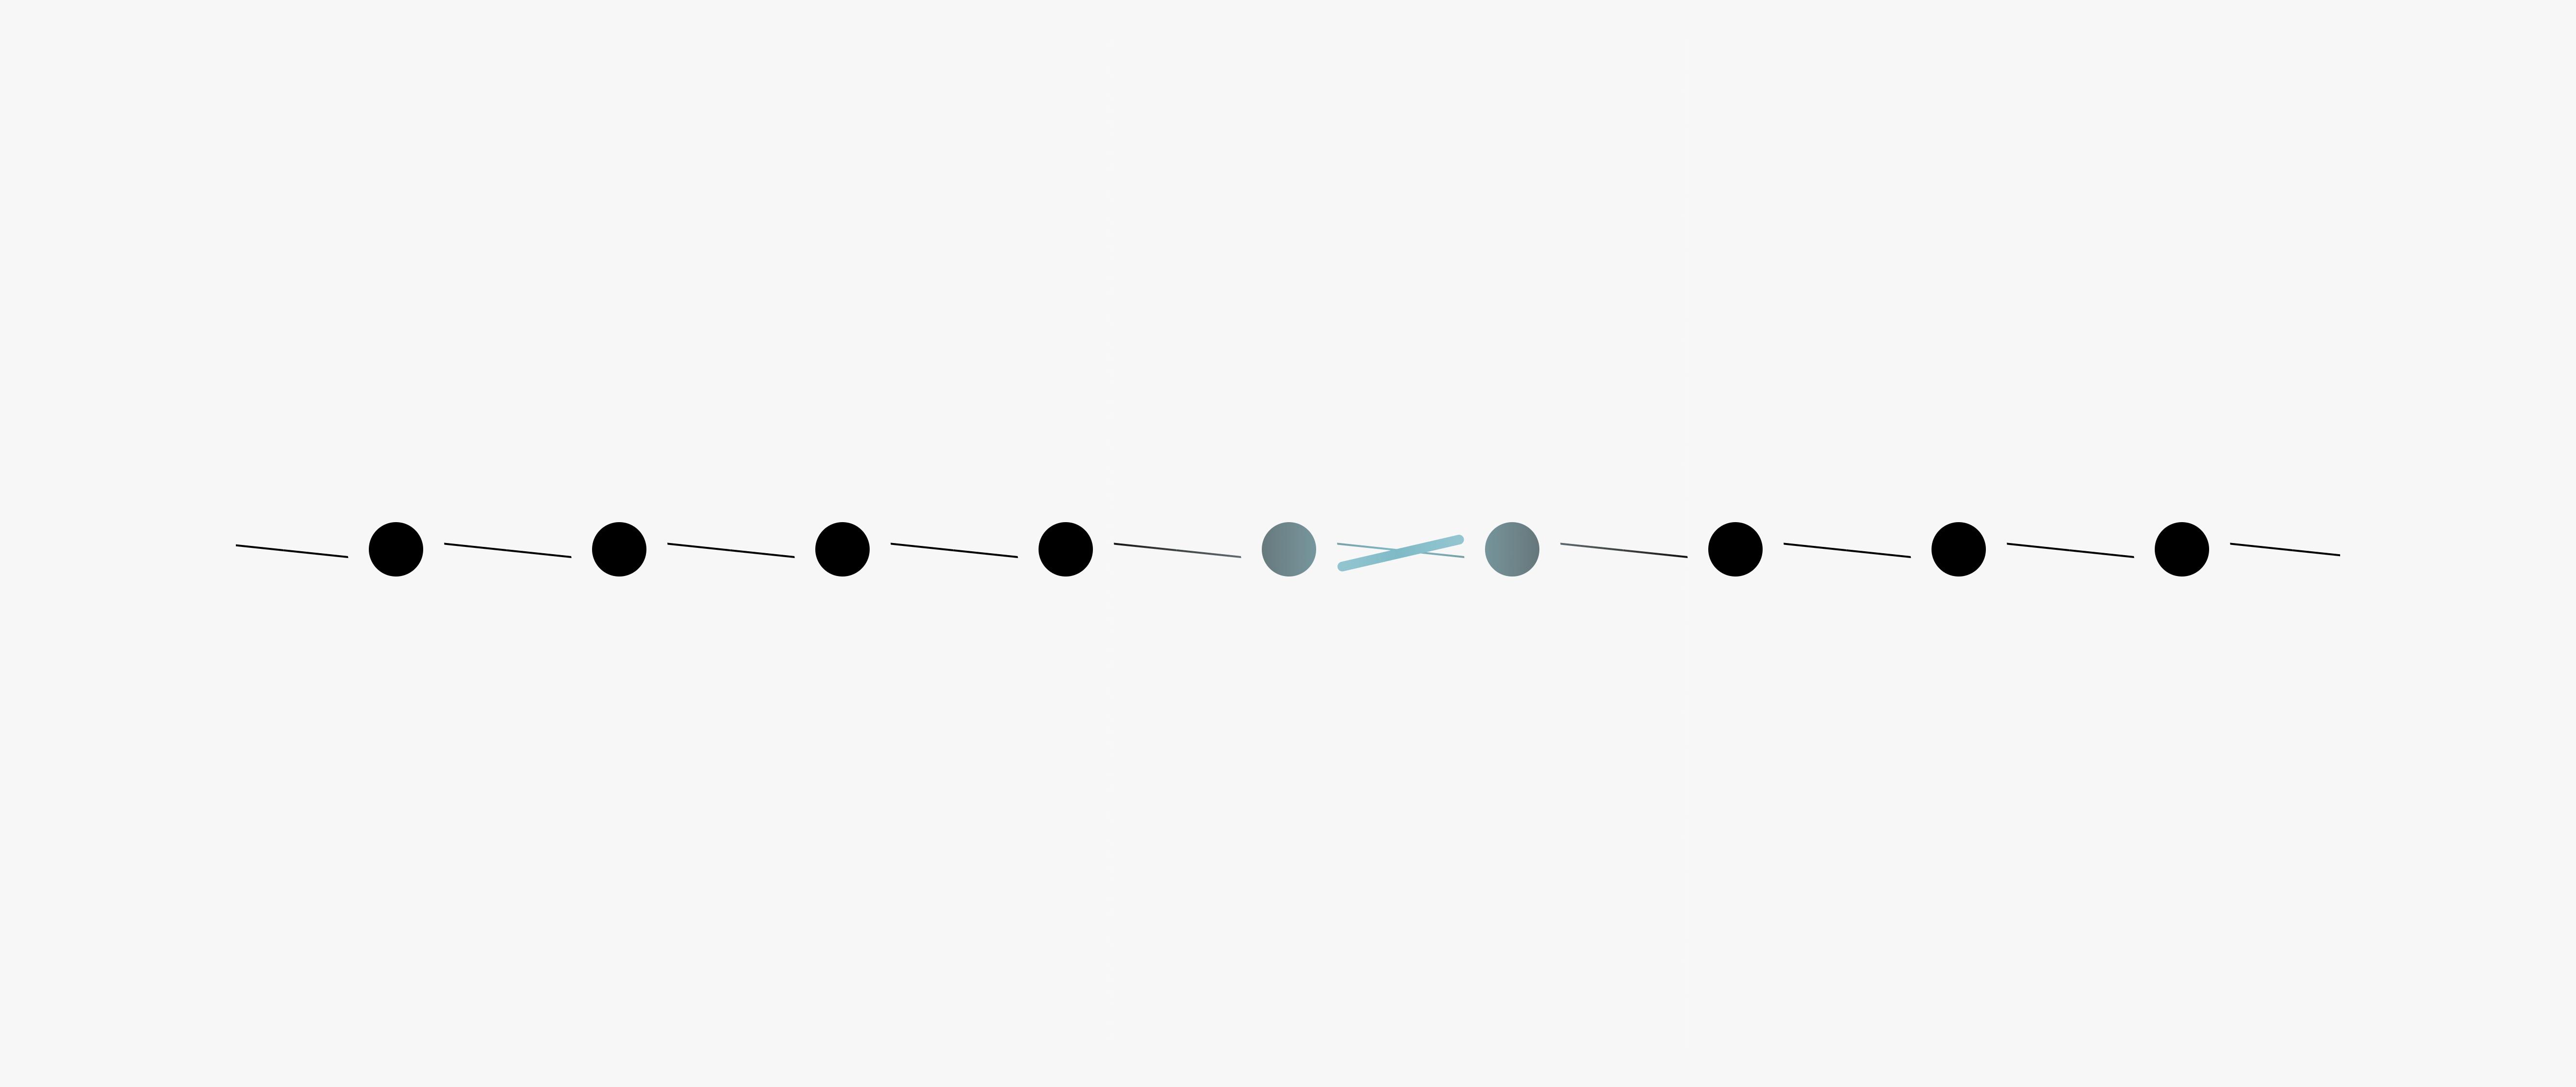
\includegraphics[width=0.8\linewidth]{media/lattice-defect.png}
  \end{figure}
  \begin{equation*}
      H = -J\sum_{n} x_nx_{n+1} - h\sum_{n}z_n + \delta H_{01}
  \end{equation*}
\end{frame}

\begin{frame}
  \frametitle{Defects in the wild}
  \framesubtitle{Using spin chains to pull out conformal defects}
  \begin{figure}
    \centering
    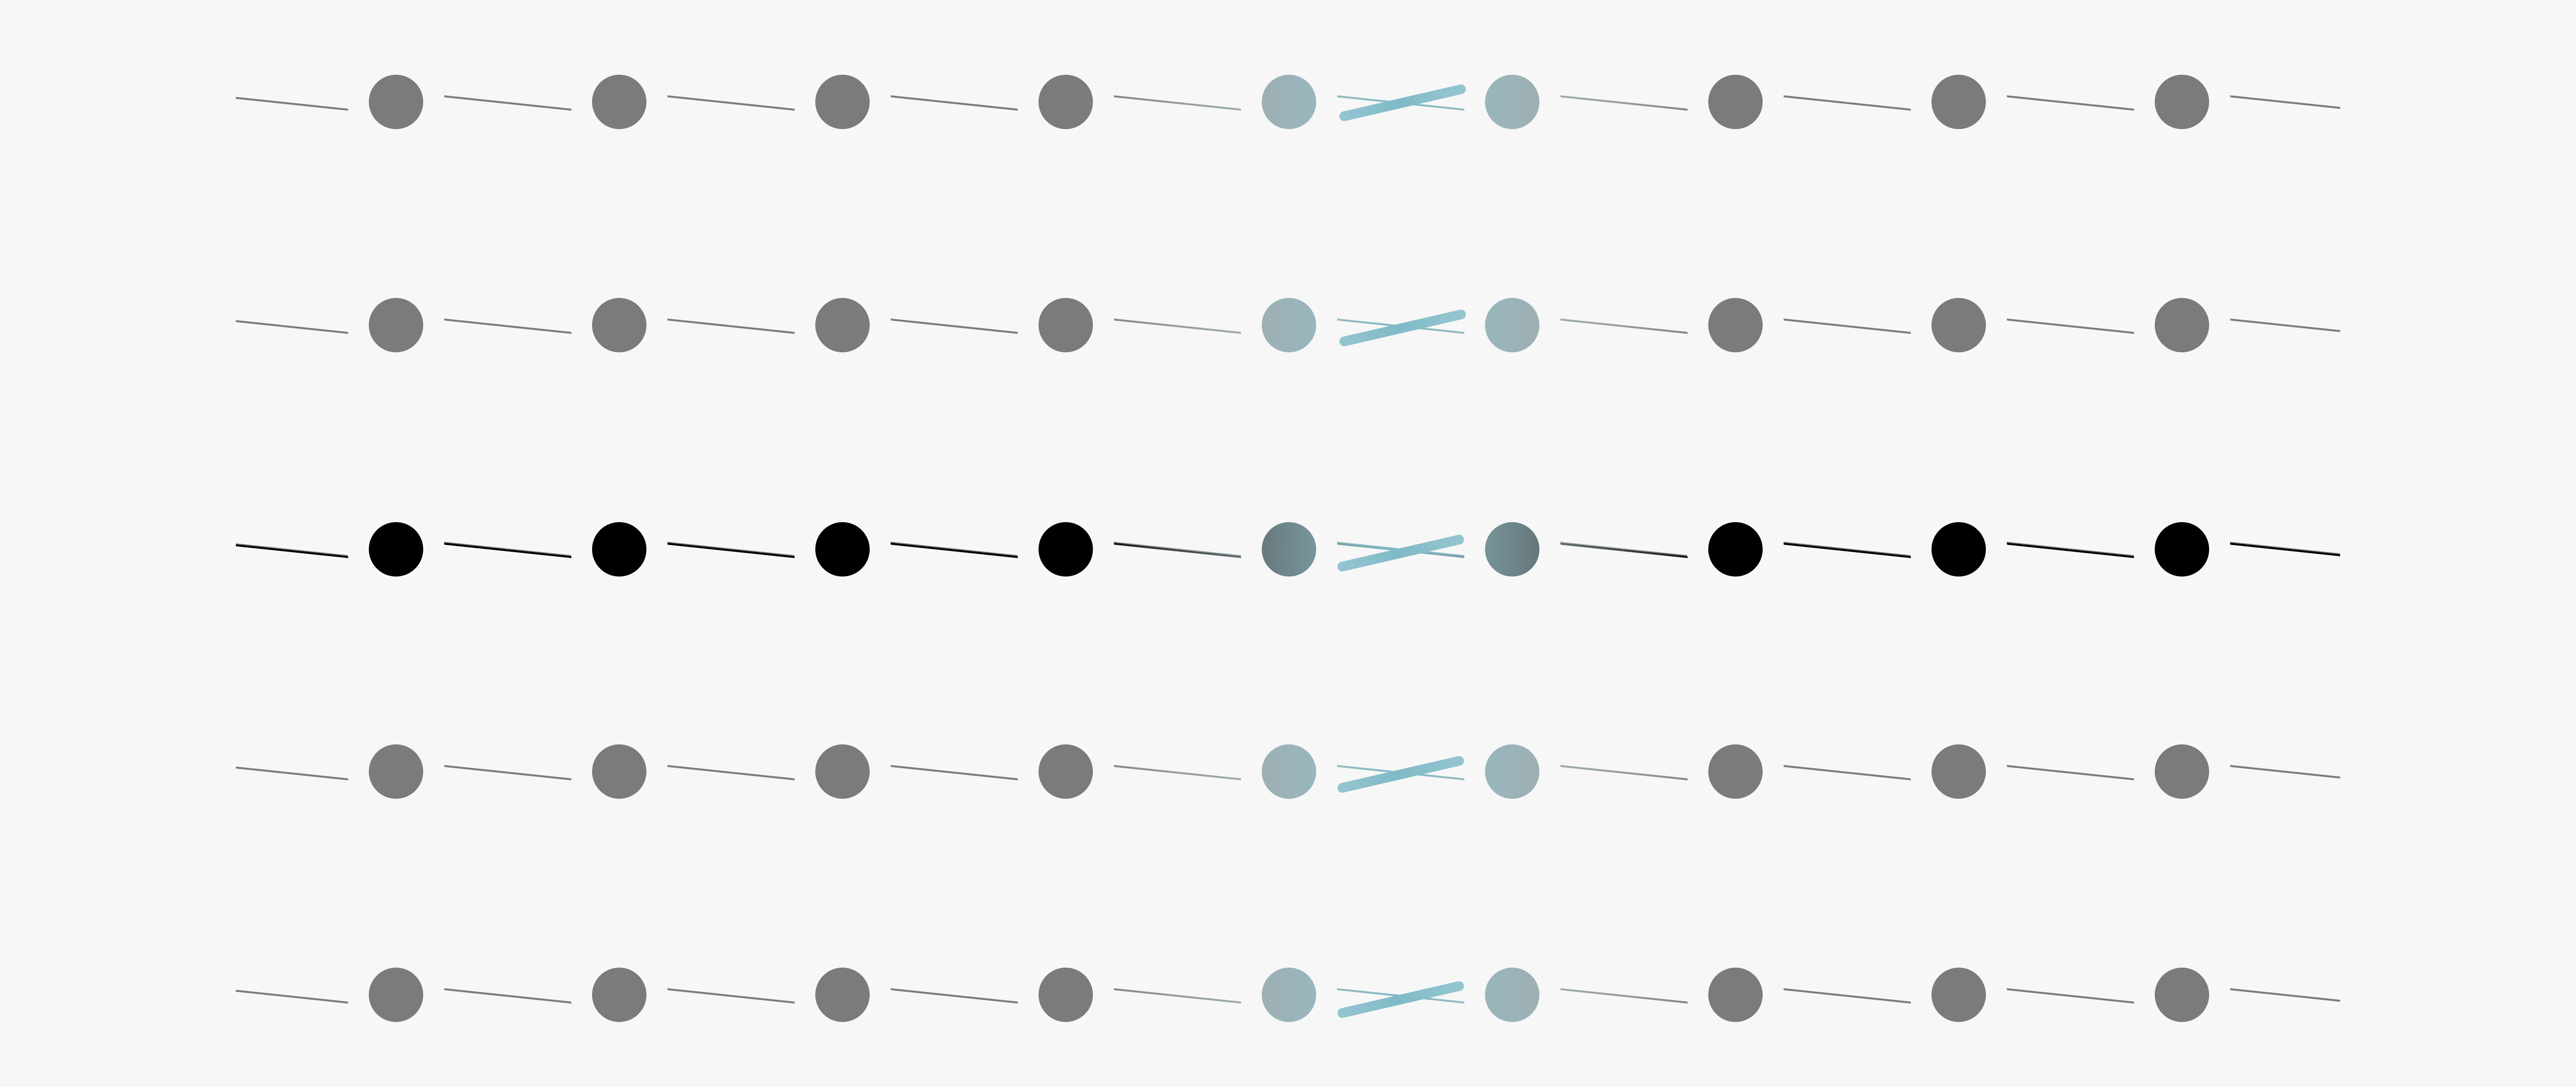
\includegraphics[width=0.8\linewidth]{media/lattice-defect-full.png}
  \end{figure}
  \begin{equation*}
      H = -J\sum_{n} x_nx_{n+1} - h\sum_{n}z_n + \delta H_{01}
  \end{equation*}
\end{frame}

\begin{frame}
  \frametitle{Defects in the wild}
  \framesubtitle{Using spin chains to pull out conformal defects}
  \begin{figure}
    \centering
    
\includegraphics[width=0.8\linewidth]{media/lattice-defect-zoom-out.png}
  \end{figure}
  \begin{equation*}
      H = -J\sum_{n} x_nx_{n+1} - h\sum_{n}z_n + \delta H_{01}
  \end{equation*}
\end{frame}

\begin{frame}
  \frametitle{Flowing with these defects}
  \framesubtitle{Chasing the next simplest case}
  \begin{columns}
    \begin{column}{0.1\paperwidth}
    \end{column}
    \begin{column}{0.35\paperwidth}
      \begin{minipage}[t][0.34\paperwidth][t]{0.35\paperwidth}
        \begin{figure}
          \centering
          \only<1>{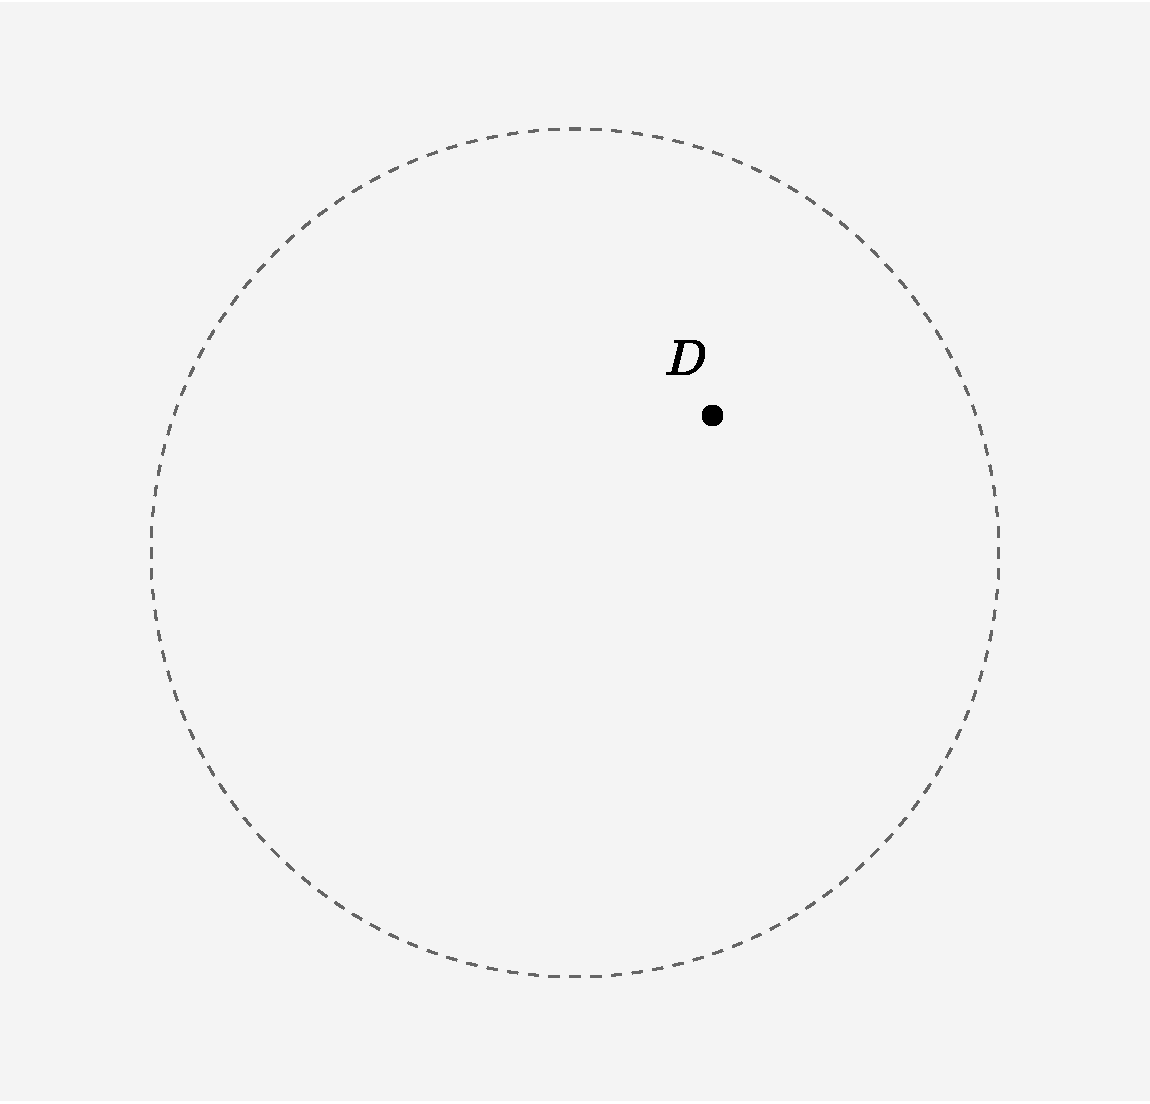
\includegraphics[width=\linewidth]{media/tricritical-flows-1}}%
          \only<2>{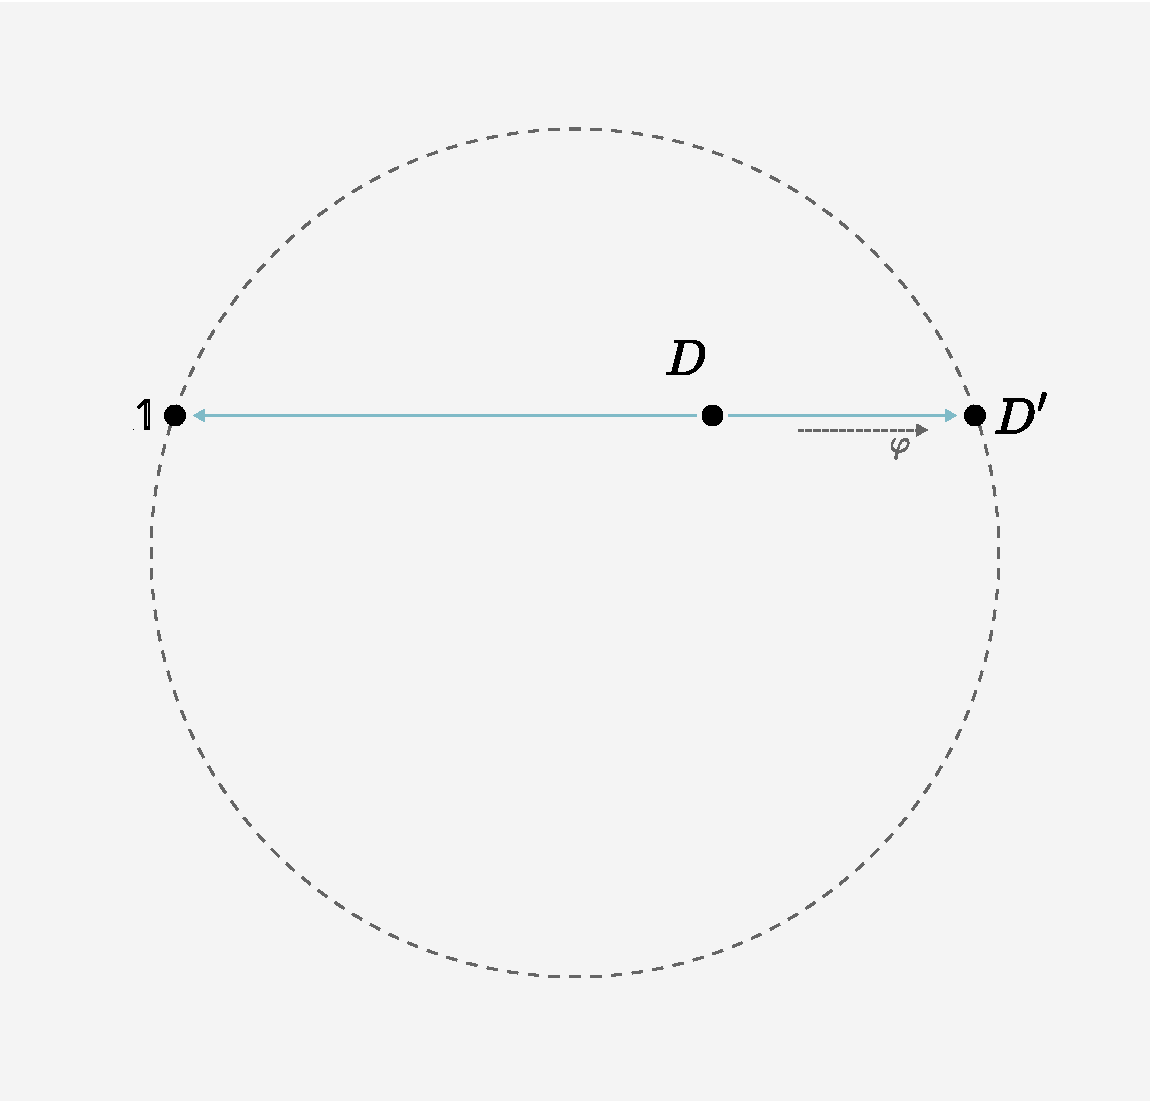
\includegraphics[width=\linewidth]{media/tricritical-flows-2}}%
          \only<3>{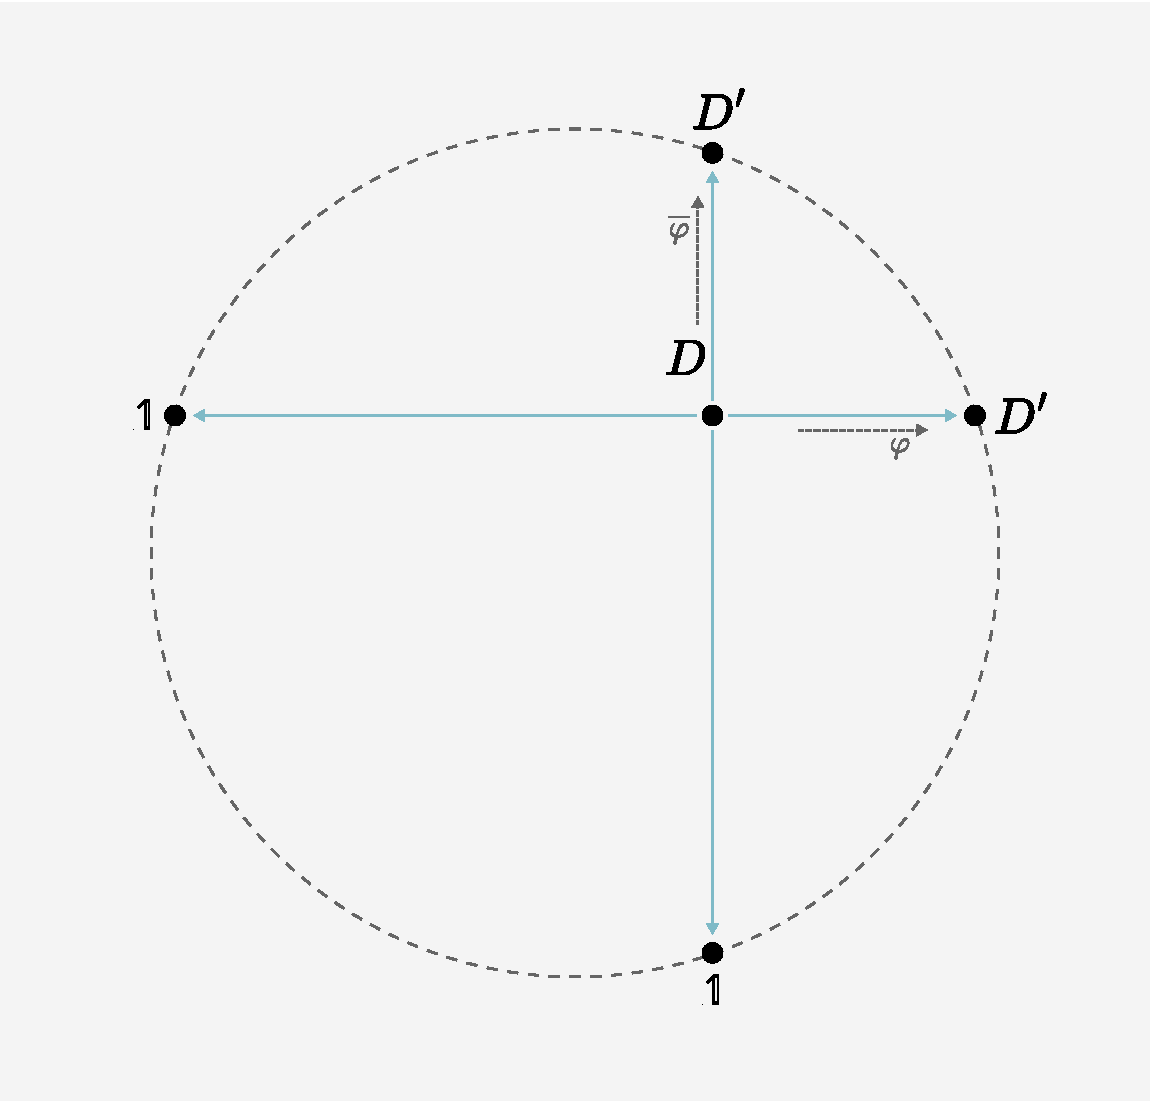
\includegraphics[width=\linewidth]{media/tricritical-flows-3}}%
          \only<4>{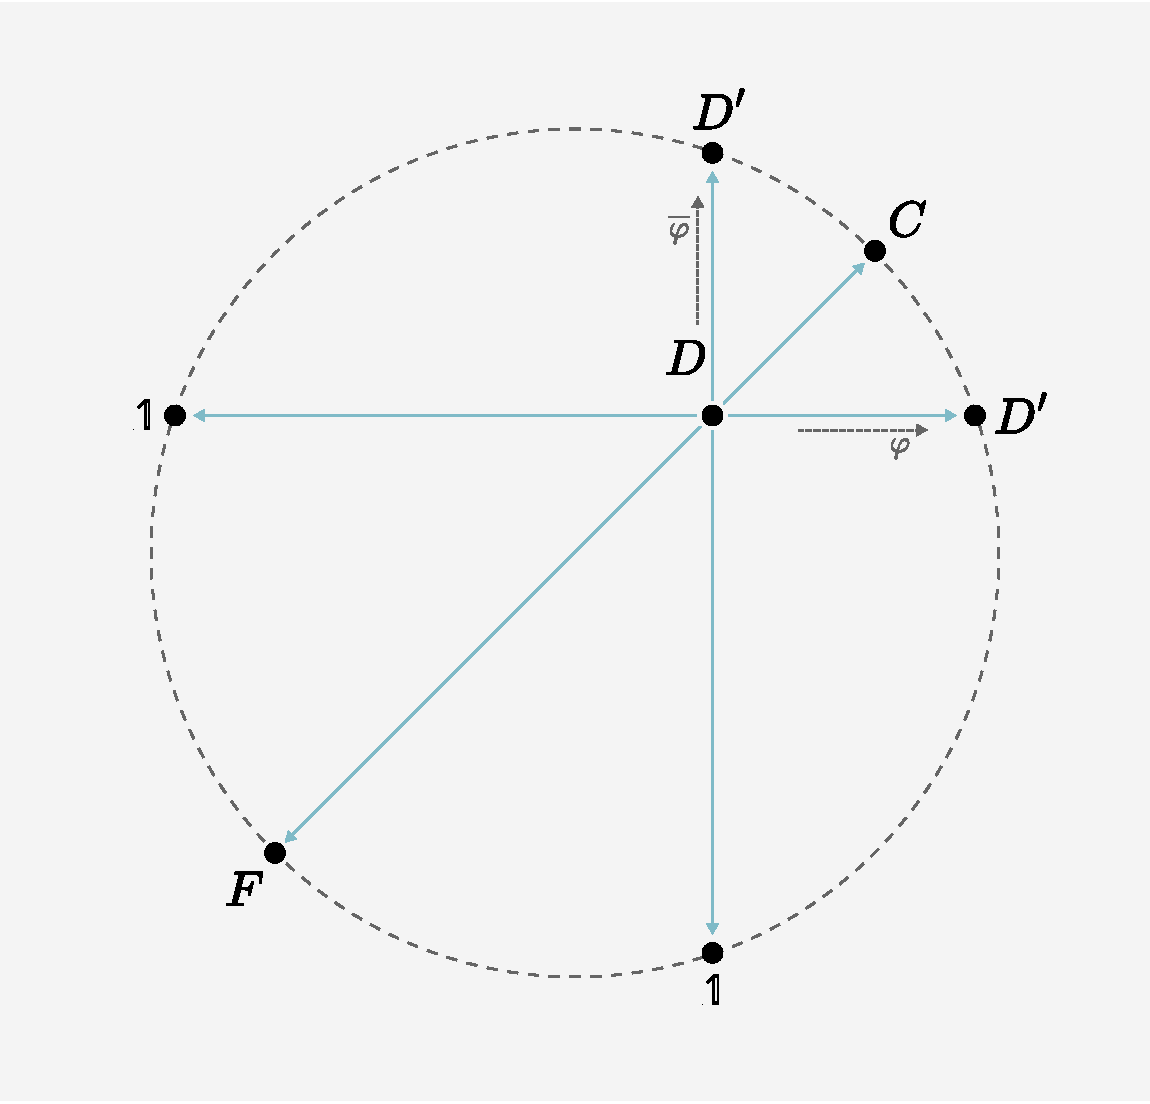
\includegraphics[width=\linewidth]{media/tricritical-flows-4}}%
          \only<5>{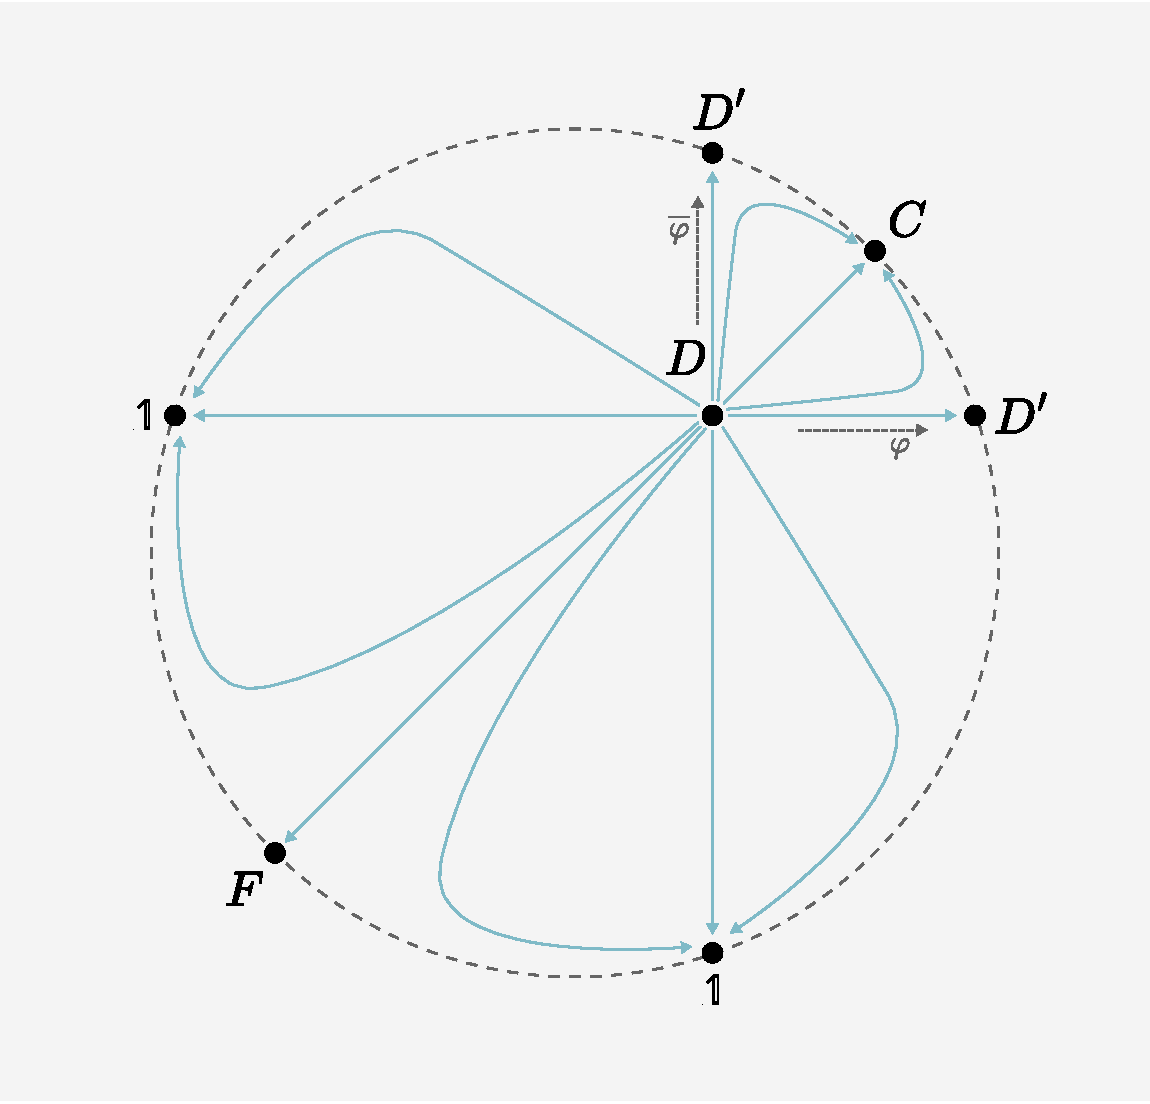
\includegraphics[width=\linewidth]{media/tricritical-flows-5}}%
        \end{figure}
      \end{minipage}
    \end{column}
    \hspace{0.02\paperwidth}%
    \begin{column}{0.45\paperwidth}%
      \begin{minipage}[t][0.34\paperwidth][t]{\linewidth}
        \raggedright
        Consider $\mathcal{T} \coloneqq M(4,5)$\par 
        \textbf{\textit{Tricritical Ising Model}}%
        \vspace{0pt plus 1fill}%
        \begin{equation*}%
          \only<1>{S = S_D}%
          \only<2>{S = S_D + \lambda_{\phi}\int_{D} \phi(z) dz}%
          \only<3>{S = S_D + \lambda_{\bar \phi}\int_{D} \bar \phi(z) dz}%
          \only<4>{S = S_D + \lambda\int_{D} \phi(z) + \bar \phi(z) dz}%
          \only<5>{S = S_D + \lambda_{\phi}\int_{D} \phi(z) dz + \lambda_{\bar \phi}\int_{D} \bar \phi(z) dz}%
        \end{equation*}
        % \vspace{0pt plus 2fill}%
        \vfill
        \raggedleft
        {\tiny Results from Watts, Runkel, and co.}
      \end{minipage}
    \end{column}
    \hspace{0.07\paperwidth}
  \end{columns}
\end{frame}

\begin{frame}
  \frametitle{Outline}
  \framesubtitle{The story so far}
  \begin{columns}[t]
    \begin{column}{0.22\textwidth}
      \centering
      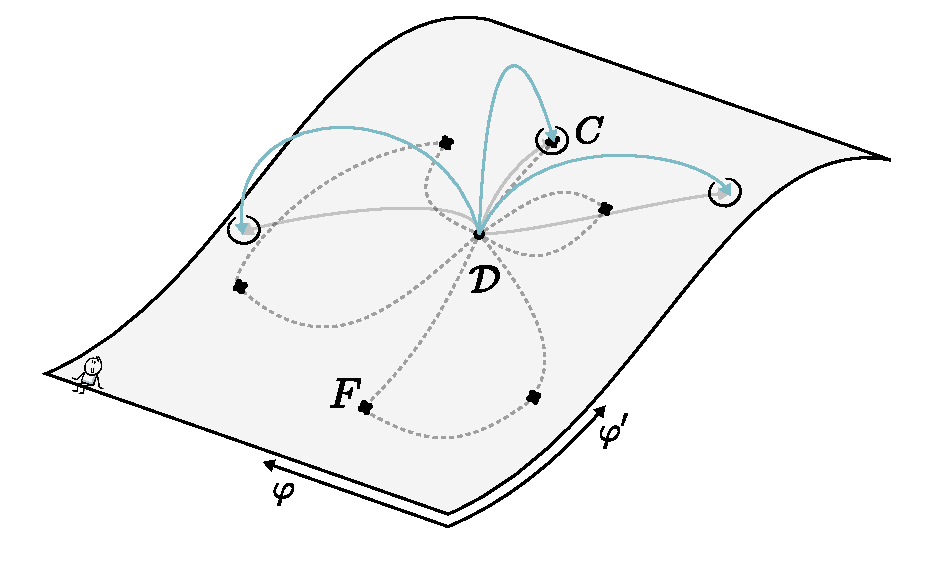
\includegraphics[width=\linewidth]{media/widget-introduction}\\[1ex]
      \tiny Motivation
    \end{column}
    \pause
    \begin{column}{0.22\textwidth}
      \centering
      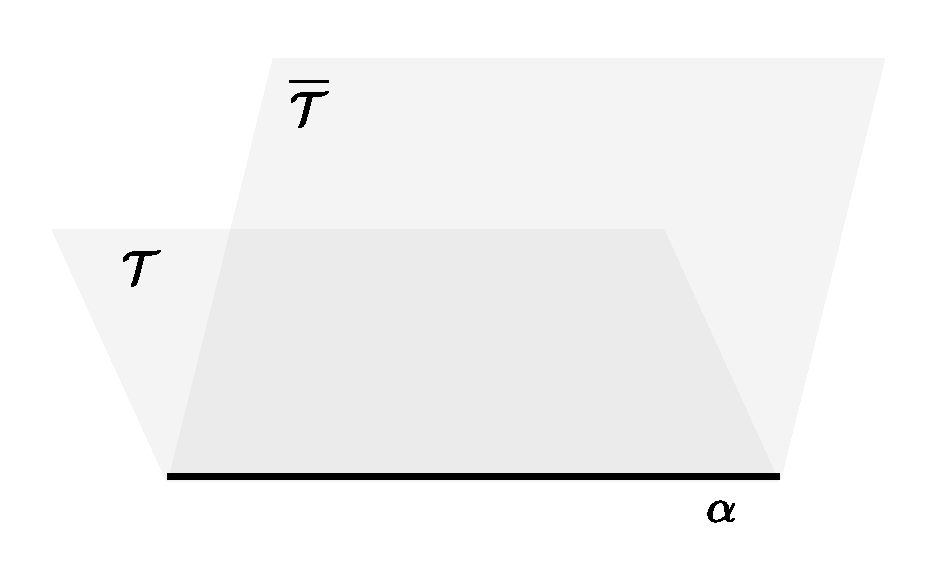
\includegraphics[width=\linewidth]{media/widget-background}\\[1ex]
      \tiny Review how to describe conformal defects
    \end{column}
    \pause
    \begin{column}{0.22\textwidth}
      \centering
      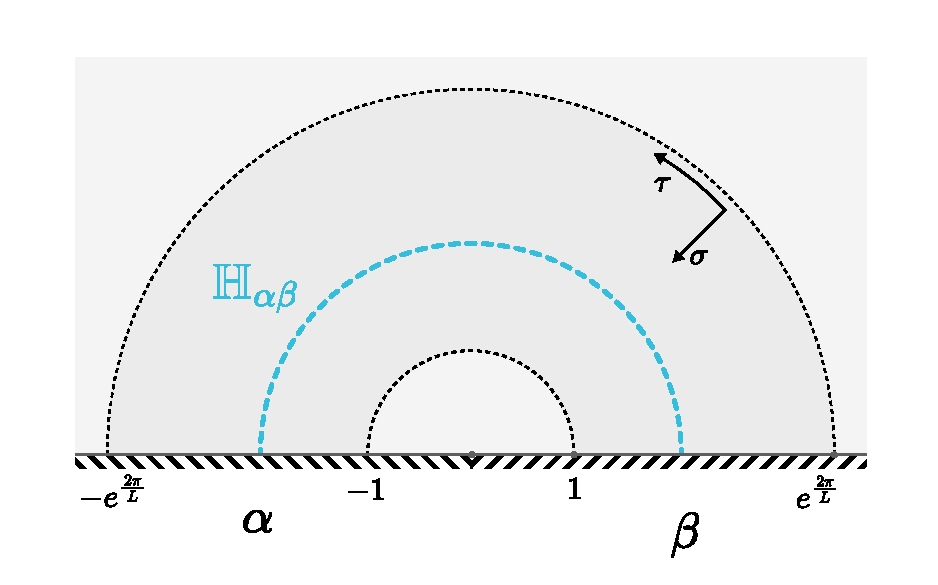
\includegraphics[width=\linewidth]{media/widget-strategy}\\[1ex]
      \tiny Approach to finding fixed points
    \end{column}
    \pause
    \begin{column}{0.22\textwidth}
      \centering
      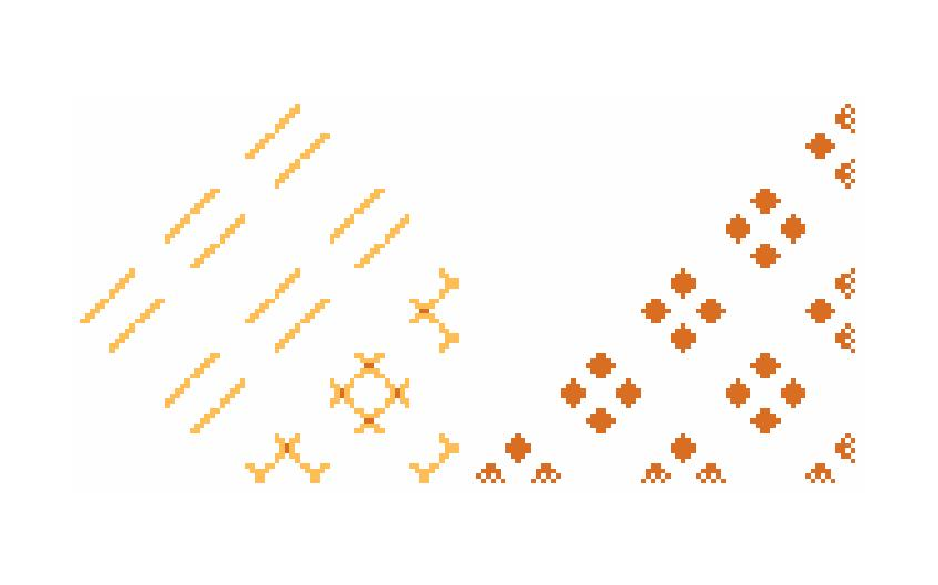
\includegraphics[width=\linewidth]{media/widget-results}\\[1ex]
      \tiny Progress and partial results
    \end{column}
  \end{columns}
\end{frame}

\begin{accentframe}{So Where are the endpoints?}{Studying the endpoints of flows by hopping and hoping.}
\end{accentframe}

\section{Finding Fixed Points}
\begin{frame}
  \frametitle{Chiral Algebras}
  \framesubtitle{The building blocks of a Conformal Field Theory}
  \centering
  \only<1-2>{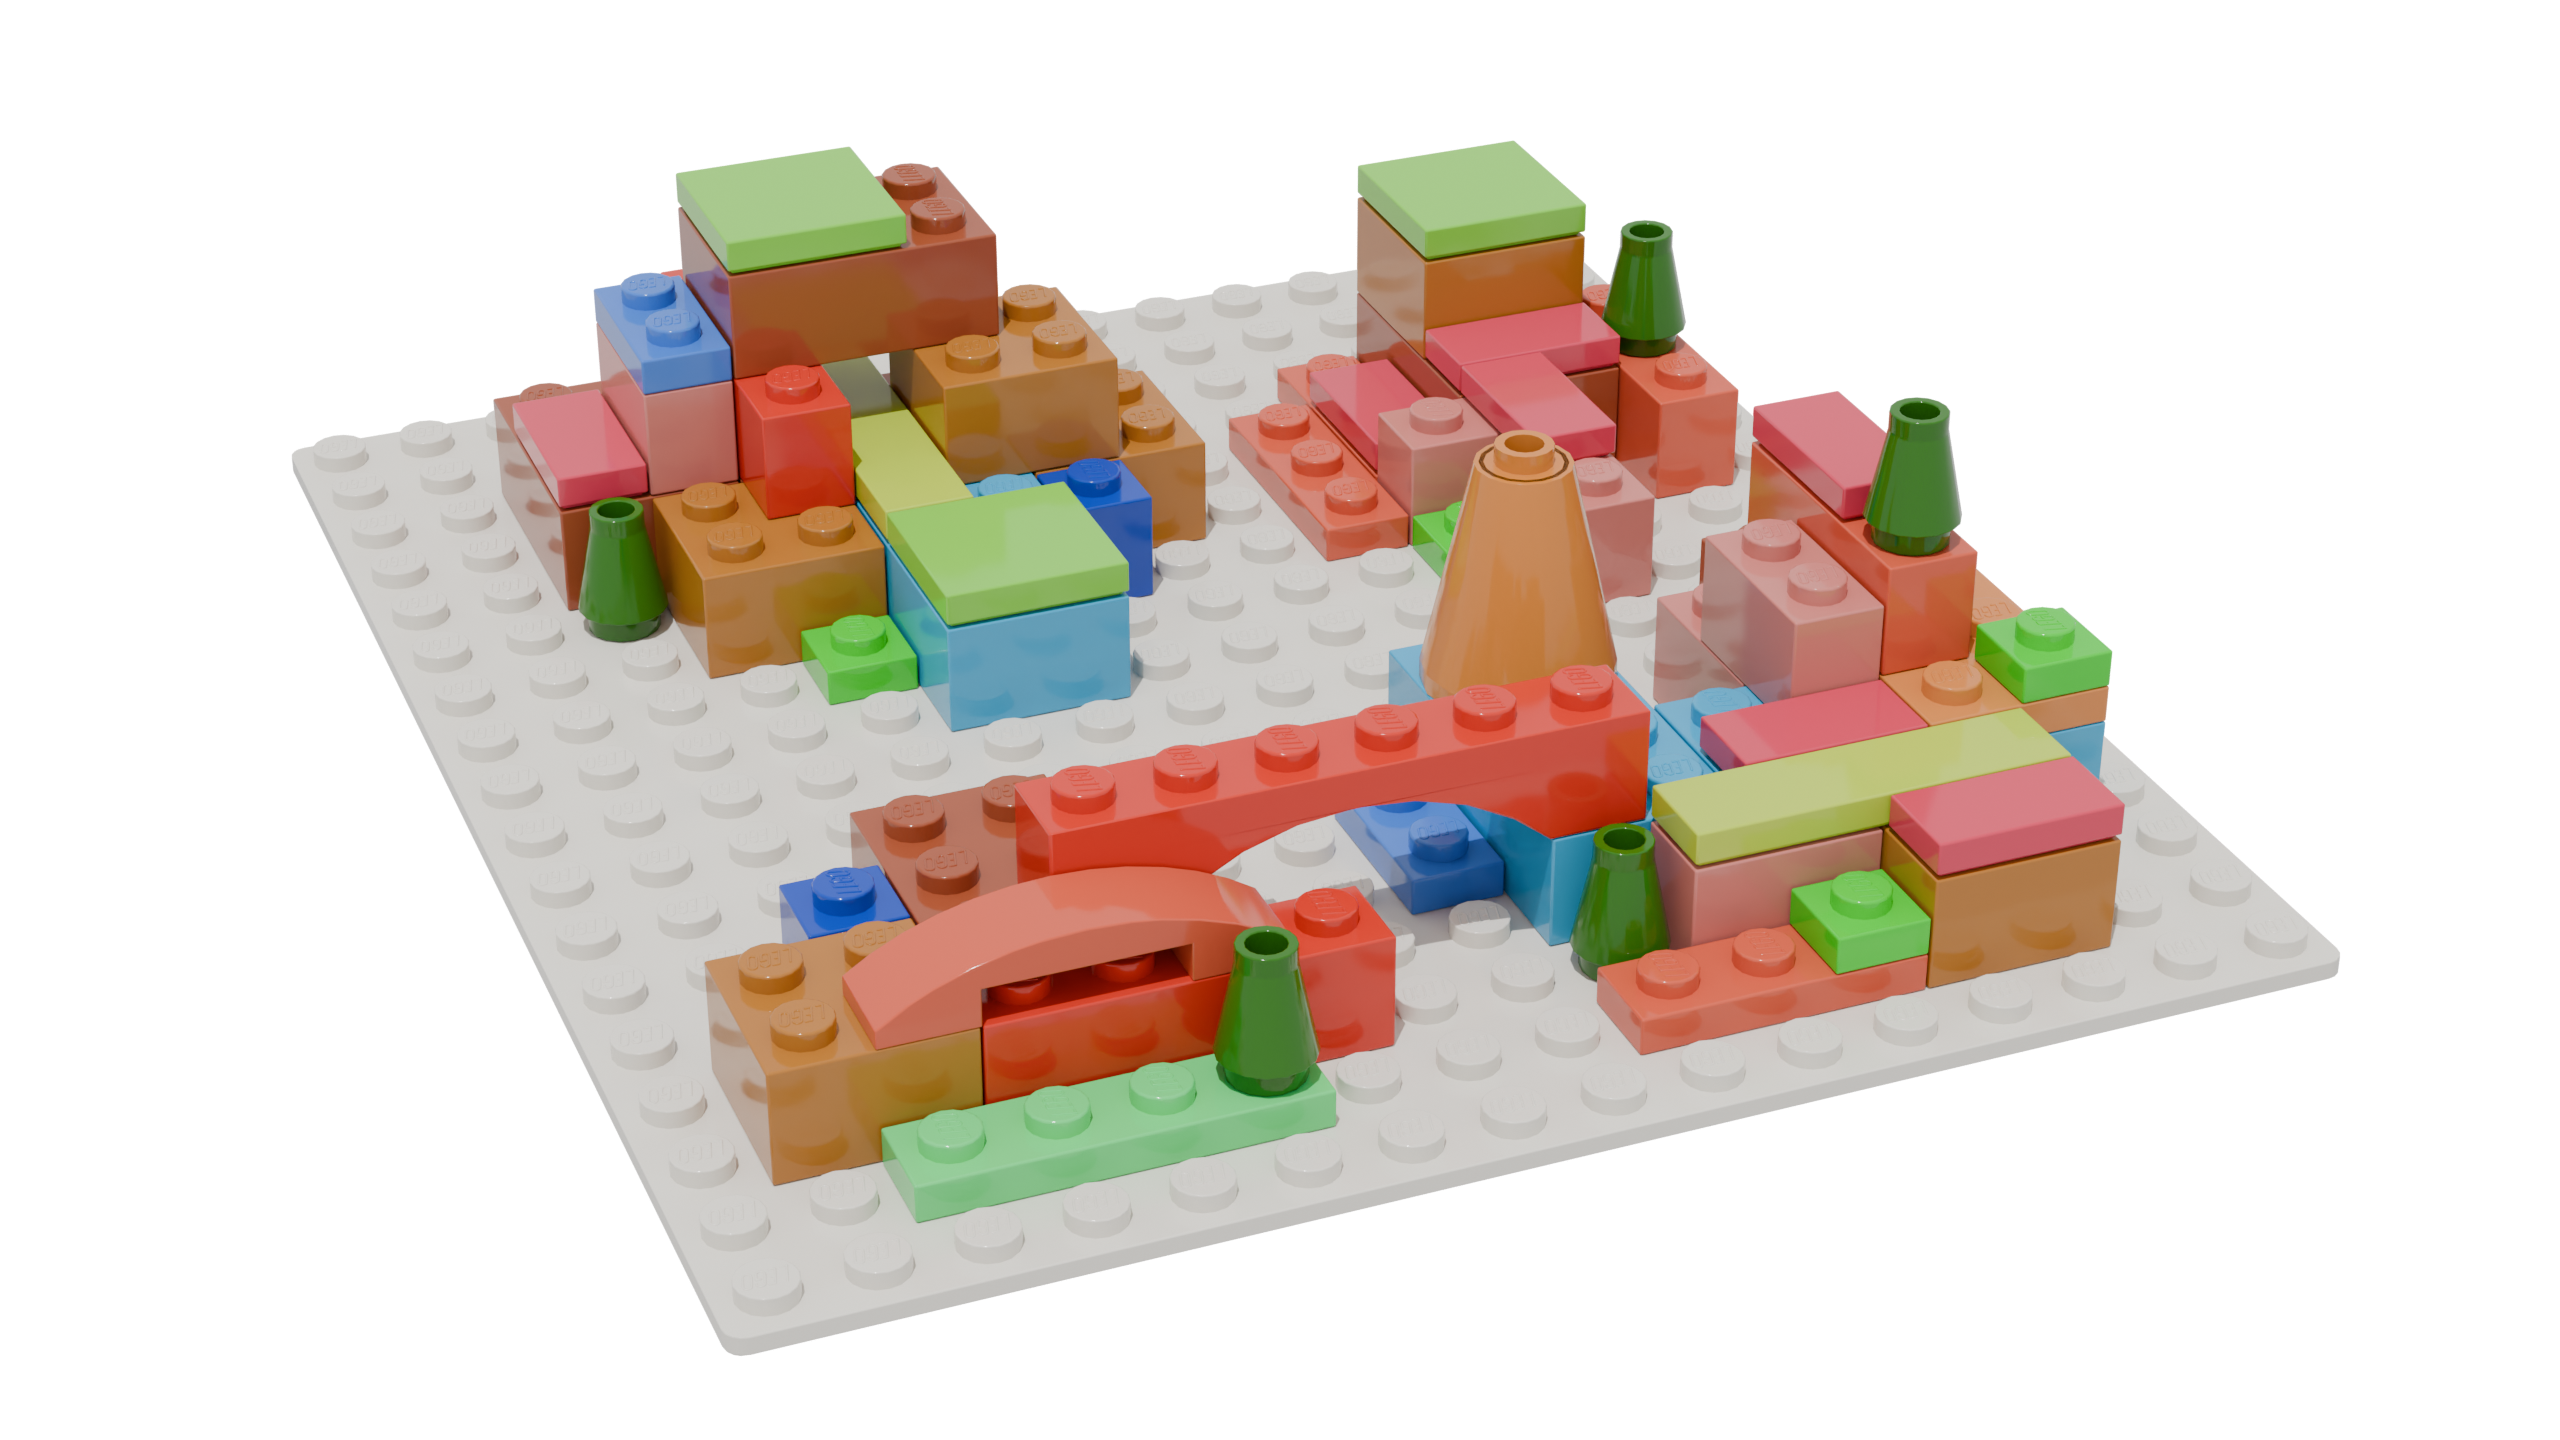
\includegraphics[width=0.6\linewidth]{media/cft-vir-lego.png}}%
  \only<3>{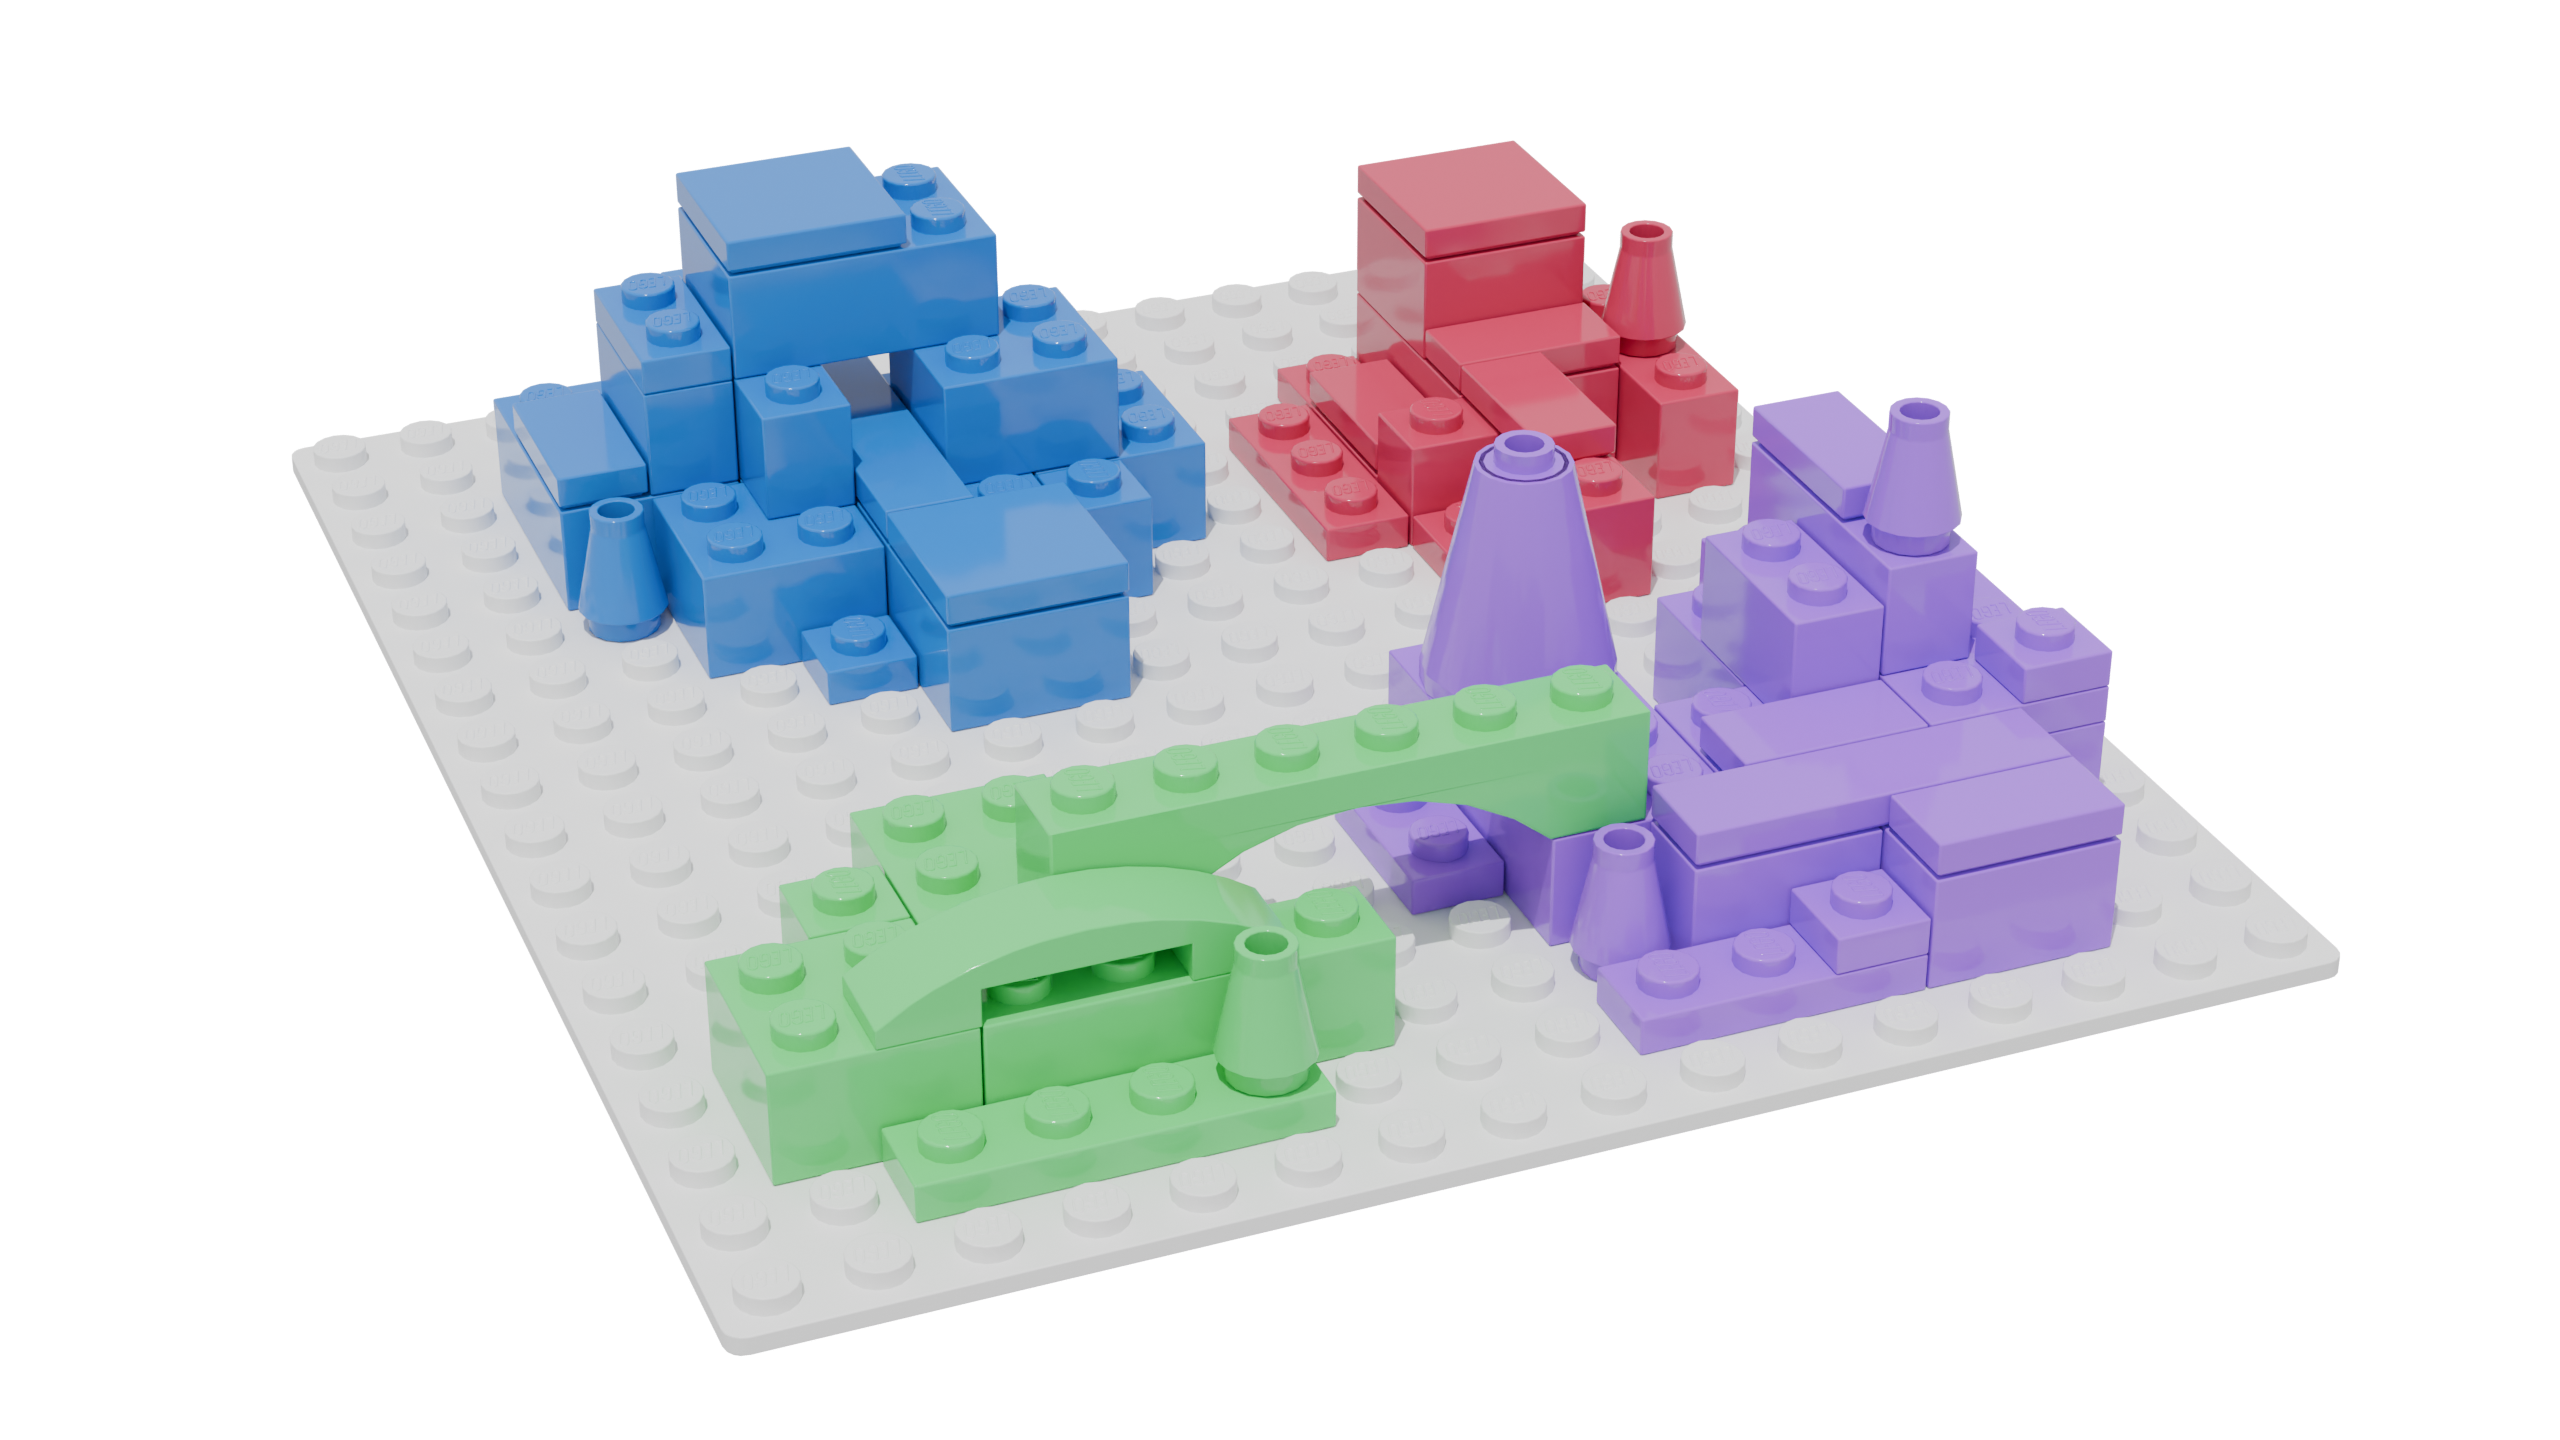
\includegraphics[width=0.6\linewidth]{media/cft-w-lego.png}}%
  \\[2ex]%
  \visible<2->{%
    \only<1-2>{
\includegraphics[width=0.7\linewidth]{media/vir-primary.pdf}}%
    \only<3>{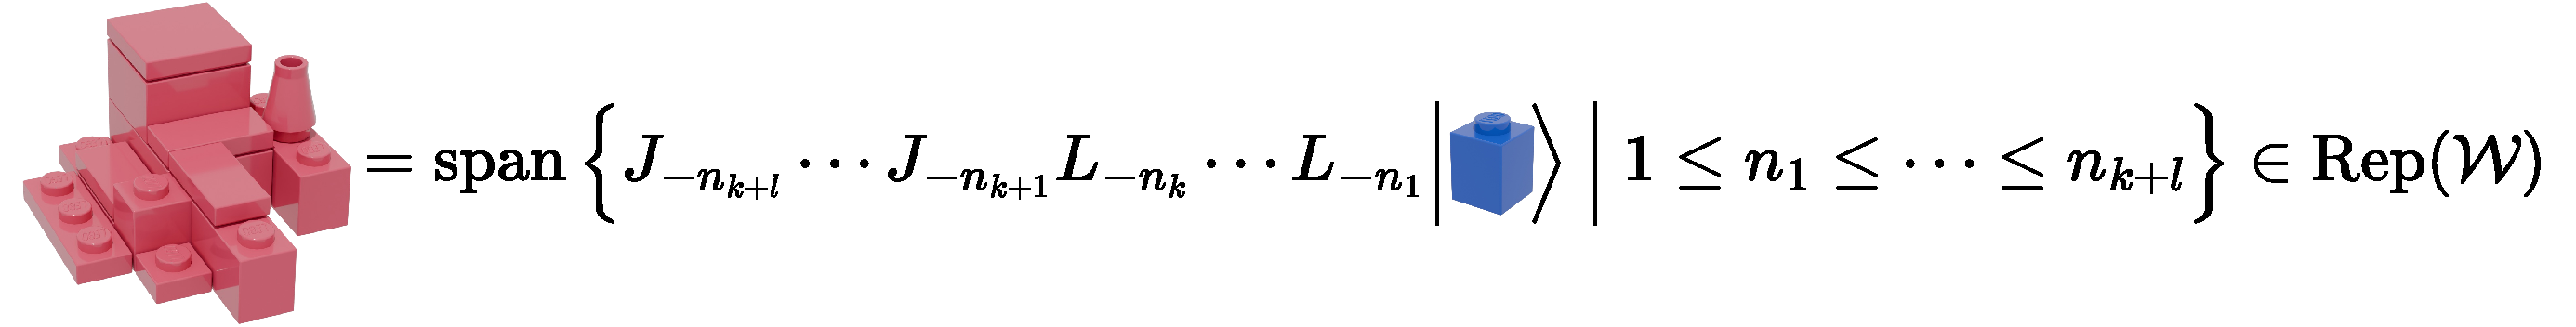
\includegraphics[width=0.7\linewidth]{media/w-primary.pdf}}%
  }
\end{frame}


\setbeamercovered{transparent}
\begin{frame}
  \frametitle{Defects are unfolded boundaries}
  \framesubtitle{Reframing the problem in terms of Boundary CFT}
  In a theory $\mathcal{T}$ with conformal defect $\alpha$, 
  \begin{figure}
    \centering
    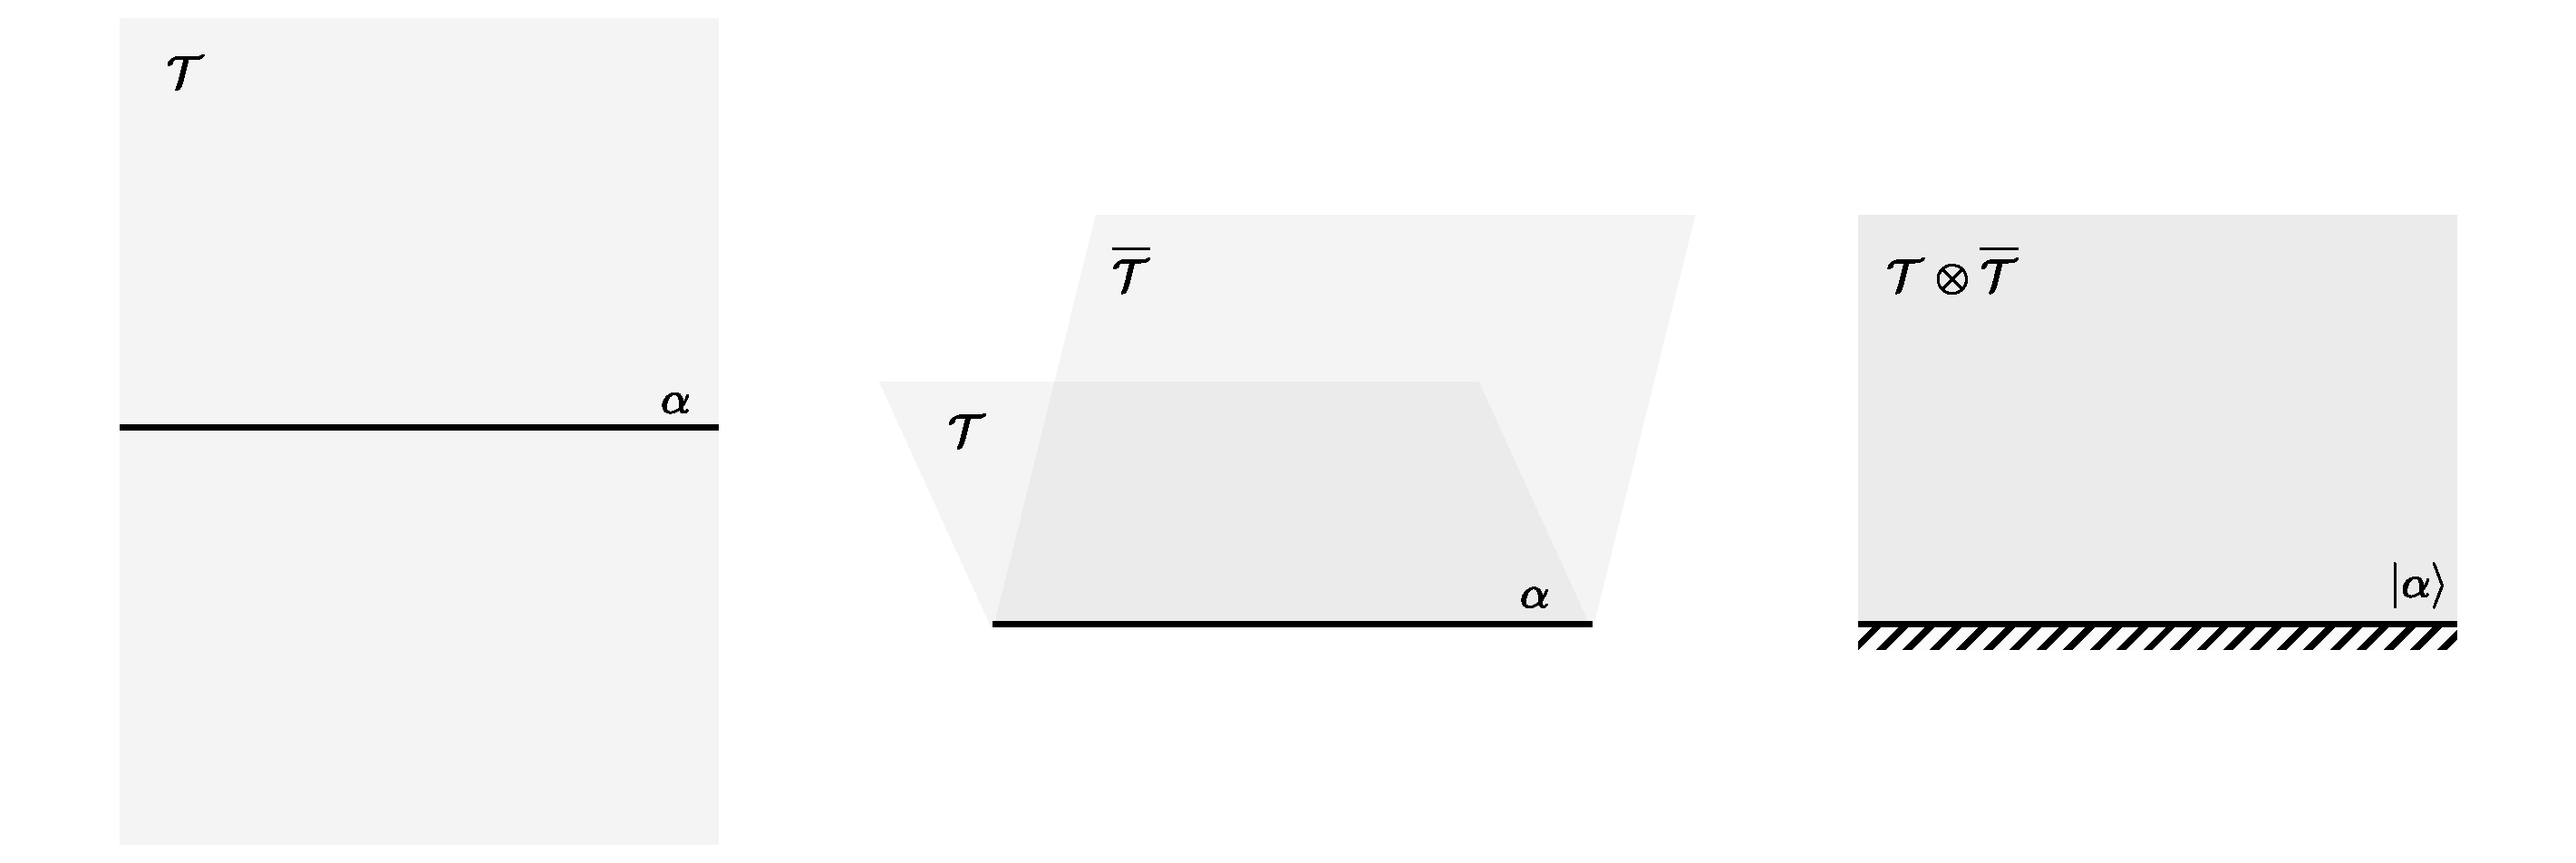
\includegraphics[width=0.9\linewidth]{media/folding-defects.pdf}
  \end{figure}
  \pause
  Similar to how a linear map
  \begin{equation}
    \alpha : \mathbb{H}\to \mathbb{H} \longleftrightarrow \ket{\alpha} : \mathbb{C}\to \mathbb{H} \otimes \mathbb{H}^\ast.
  \end{equation}
\end{frame}

\begin{frame}
  \frametitle{Characterizing Conformal Defects}
  \framesubtitle{Useful tools}
  Invariance under translation along the defect implies
  \begin{equation}
    T_{\rm{above}}(z) - \bar T_{\rm{above}}(\bar z) = 
    T_{\rm{below}}(z) - \bar T_{\rm{below}}(\bar z)
  \end{equation}
  \pause
  For a boundary state $\alpha$ this translates to 
  \begin{equation}
    (L_n - \bar L_{-n})\ket{\alpha} = 0.
  \end{equation}
\end{frame}

\begin{frame}
  \frametitle{Characterizing Conformal Defects}
  \framesubtitle{Useful tools}
  The condition
  \begin{equation}
    (L_n - \bar L_{-n})\ket{\alpha} = 0,
  \end{equation}
  implies that...

  \begin{minipage}[t][0.5\textheight][t]{\linewidth}
    \only<1>{
      \begin{block}{Fact I}
        Boundary states are built with spinless primaries since for $n=0$
        \begin{equation}
          (L_0 - \bar L_0) \ket{\alpha} = 0 
        \end{equation}
      \end{block}
    }
    \only<2>{
      \begin{block}{Fact II}
        A basis is given by \textbf{Ishibashi states} $|i\rangle\!\rangle$ defined for a spinless primary $i$ by
        \begin{equation}
          |i\rangle\!\rangle = \sum_{n} |i,n\rangle \otimes U |i,n\rangle,
        \end{equation}with $|i,n\rangle$ an orthonormal basis of the $i$ irrep, and $U$ fixed antiunitary map.
      \end{block}
    }
    \only<3>{
      \begin{block}{Fact III}
        Each boundary state is given by 
        \begin{equation}
          \ket{\alpha} = \sum_{h_i = \bar h_i}\alpha_i|i\rangle\!\rangle,
        \end{equation}
        for some $\alpha_i \in \mathbb{C}$.
      \end{block}
    }
  \end{minipage}
\end{frame}

\begin{frame}
  \frametitle{Strategy}
  \framesubtitle{How can we then find fixed points?}
  \begin{columns}[t]
    \begin{column}{0.35\textwidth}
      \centering
      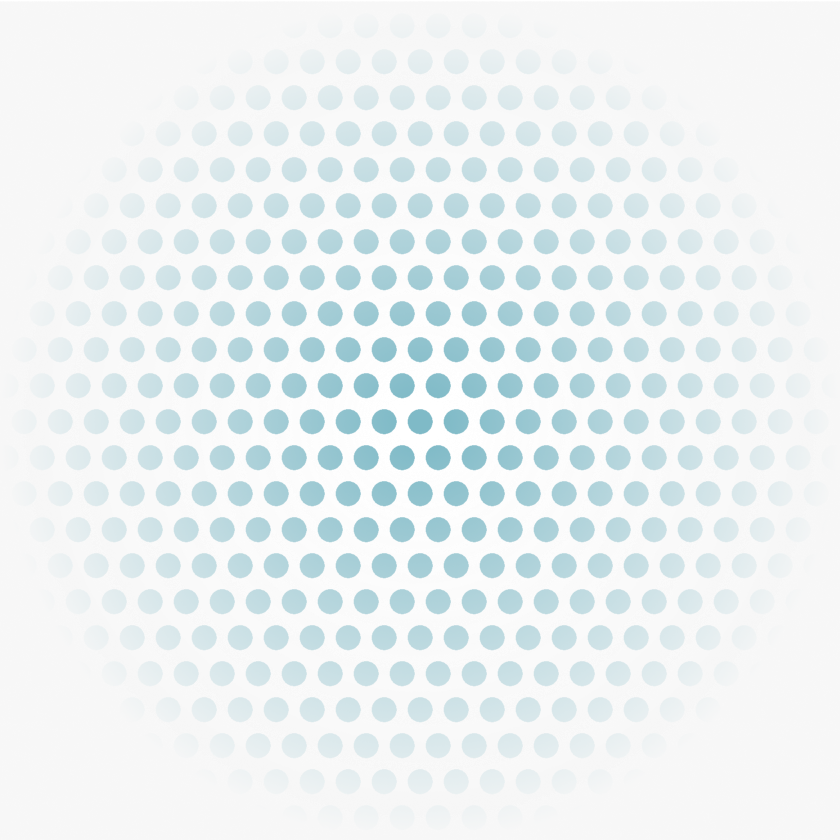
\includegraphics[width=0.2\paperwidth, trim=0 0 0 2pt, clip]{media/widget-calculate.png}\\[1ex]
      \footnotesize Find a way to generate conformal defects.
    \end{column}
    \pause
    \begin{column}{0.35\textwidth}
      \centering
      \only<1>{\transparent{0.3}
\includegraphics[width=0.2\paperwidth, trim=0 0 0 2pt, clip]{media/widget-constrain.png}\\[1ex]}%
      \only<2>{
\includegraphics[width=0.2\paperwidth, trim=0 0 0 2pt, clip]{media/widget-constrain.png}\\[1ex]}%
      \footnotesize Use constraints to check which ones could be the fixed point.
    \end{column}
  \end{columns}
\end{frame}

\begin{accentframe}{Finding Defect Builders}{A story of cheating using rational theories and gauging.}
\end{accentframe}

\section{Generate Defects}
\begin{frame}
  \frametitle{Cardy Trick}
  \framesubtitle{A cheeky way to generate boundaries}
  \centering
  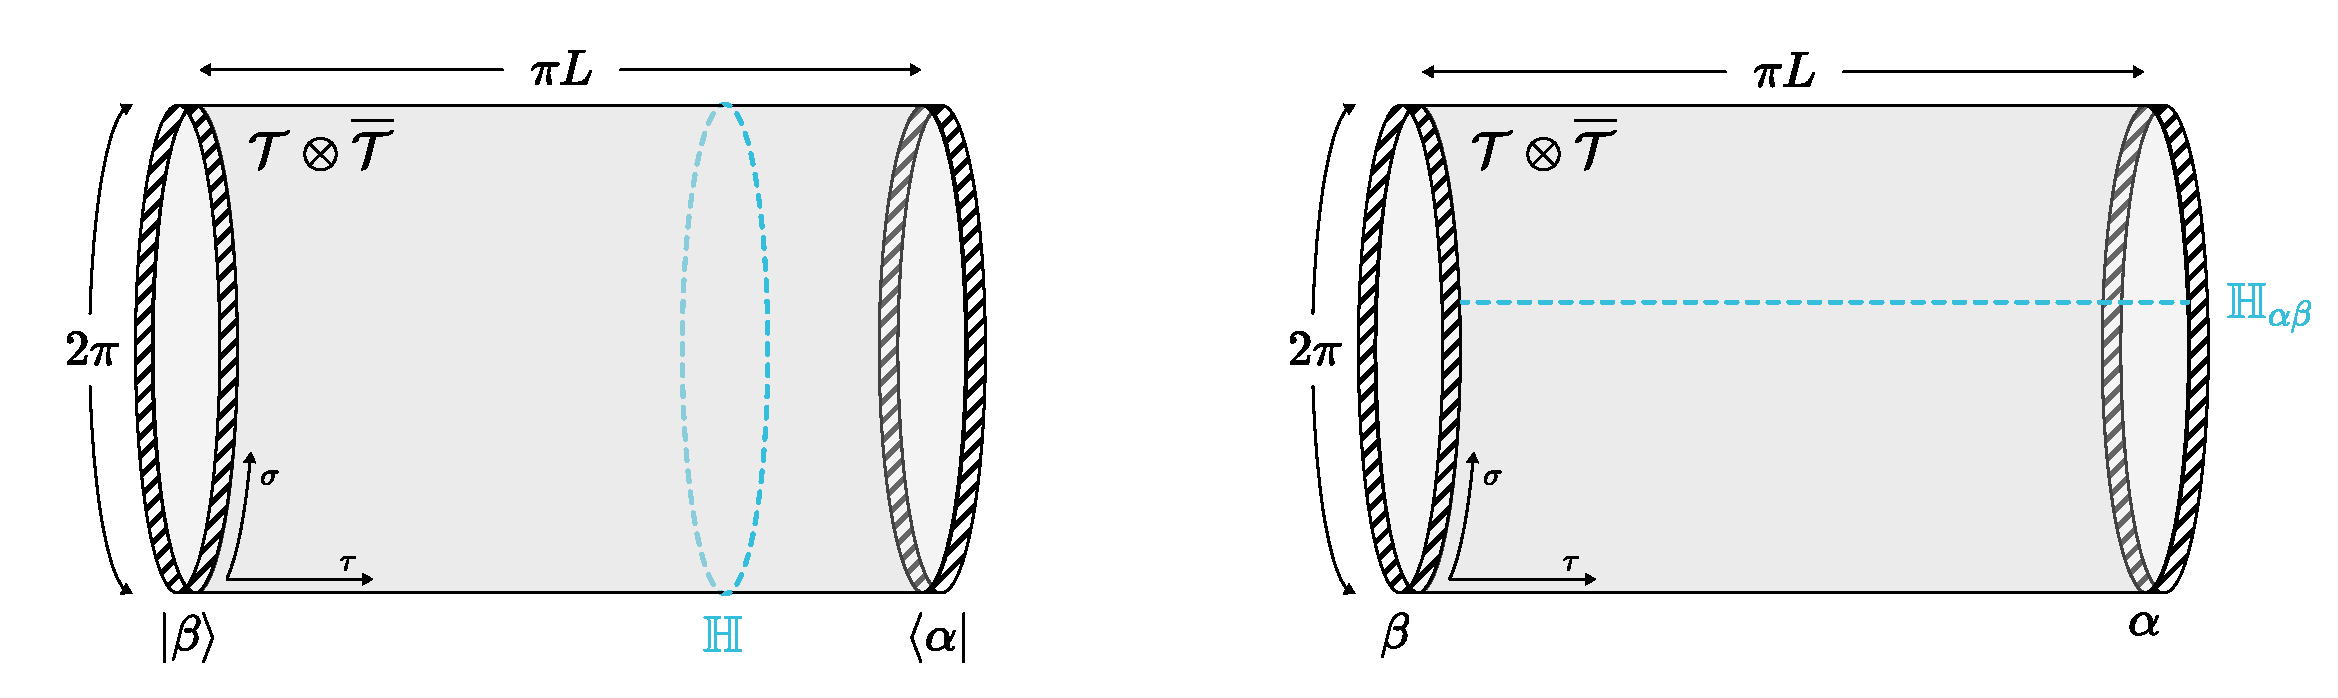
\includegraphics[width=0.8\linewidth]{media/open-closed-string-duality.pdf}
  \pause
  \begin{block}{Cardy's Condition}
    Equating the channels we have
    \begin{equation}
      \langle \alpha, e^{-\pi L H_{\tau}} \beta\rangle = Z(L) = \mathrm{Tr\,}_{\mathbb{H}_{\alpha \beta}}e^{- 2\pi H_\sigma}
    \end{equation}
  \end{block}
\end{frame}

\begin{frame}
  \frametitle{Cardy Trick}
  \framesubtitle{A cheeky way to generate boundaries}
  \begin{columns}
    \begin{column}{0.6\textwidth}
      \raggedright
      We can project into an annulus with Hamiltonian
      \begin{equation}
        H_\tau = L_0 + \bar L_0 - \frac{c}{12},
      \end{equation}
      and partition function
      \begin{equation}
        Z(L) = \langle \alpha, e^{-\pi L \left(L_0 + \bar L_0 - \frac{c}{12} \right)} \beta \rangle.
      \end{equation}
    \end{column}
    \begin{column}{0.4\textwidth}
    \end{column}
    \begin{textblock*}{0.38\textwidth}(0.6\textwidth+0.15\paperwidth, 0.00\paperheight)
      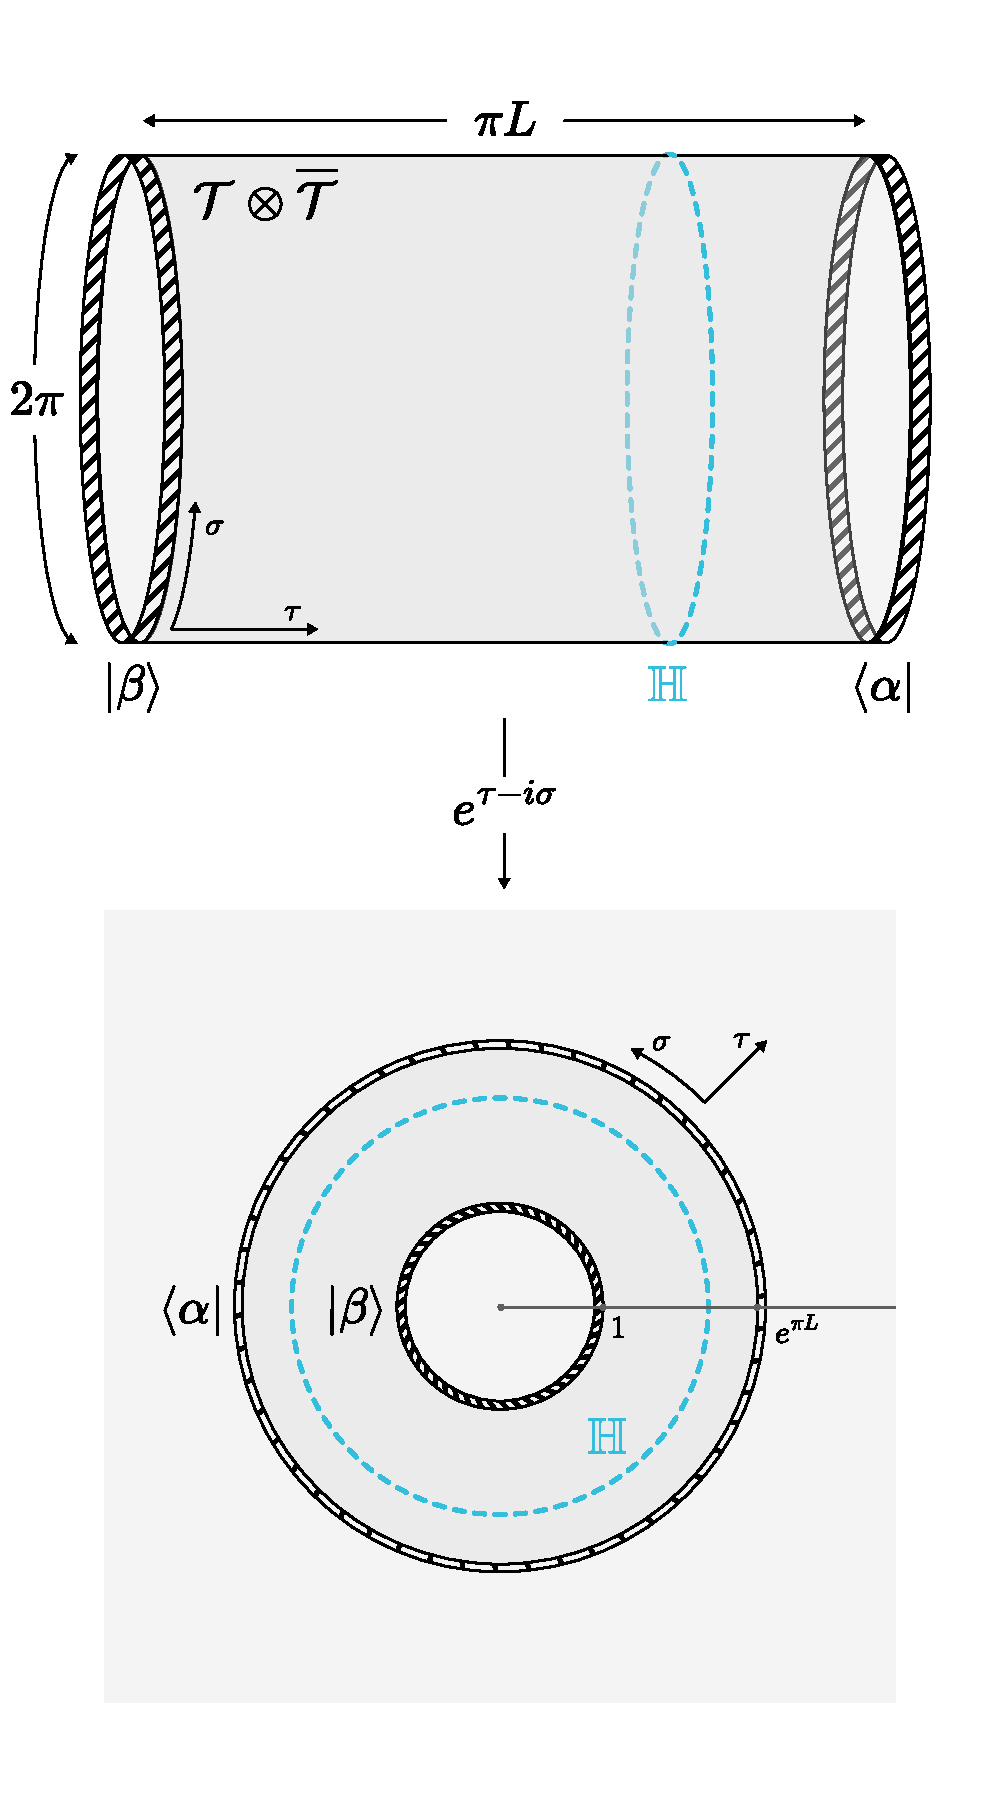
\includegraphics[width=\linewidth]{media/annulus.pdf}
    \end{textblock*}
  \end{columns}
\end{frame}

\begin{frame}
  \frametitle{Cardy Trick}
  \framesubtitle{A cheeky way to generate boundaries}
  \begin{columns}
    \begin{column}{0.6\textwidth}
      \raggedright
      But also onto an upper half plane with Hamiltonian
      \begin{equation}
        H_\sigma = -\frac{1}{L} \left(L_0  - \frac{c}{24}\right),
      \end{equation}
      and partition function
      \begin{equation}
        Z(L) = \mathrm{Tr}_{\mathbb{H}_{\alpha \beta}} e^{\frac{2\pi}{L} \left( L_0 - \frac{c}{12} \right)}.
      \end{equation}
    \end{column}
    \begin{column}{0.4\textwidth}
    \end{column}
    \begin{textblock*}{0.42\textwidth}(0.6\textwidth+0.14\paperwidth, 0.00\paperheight)
      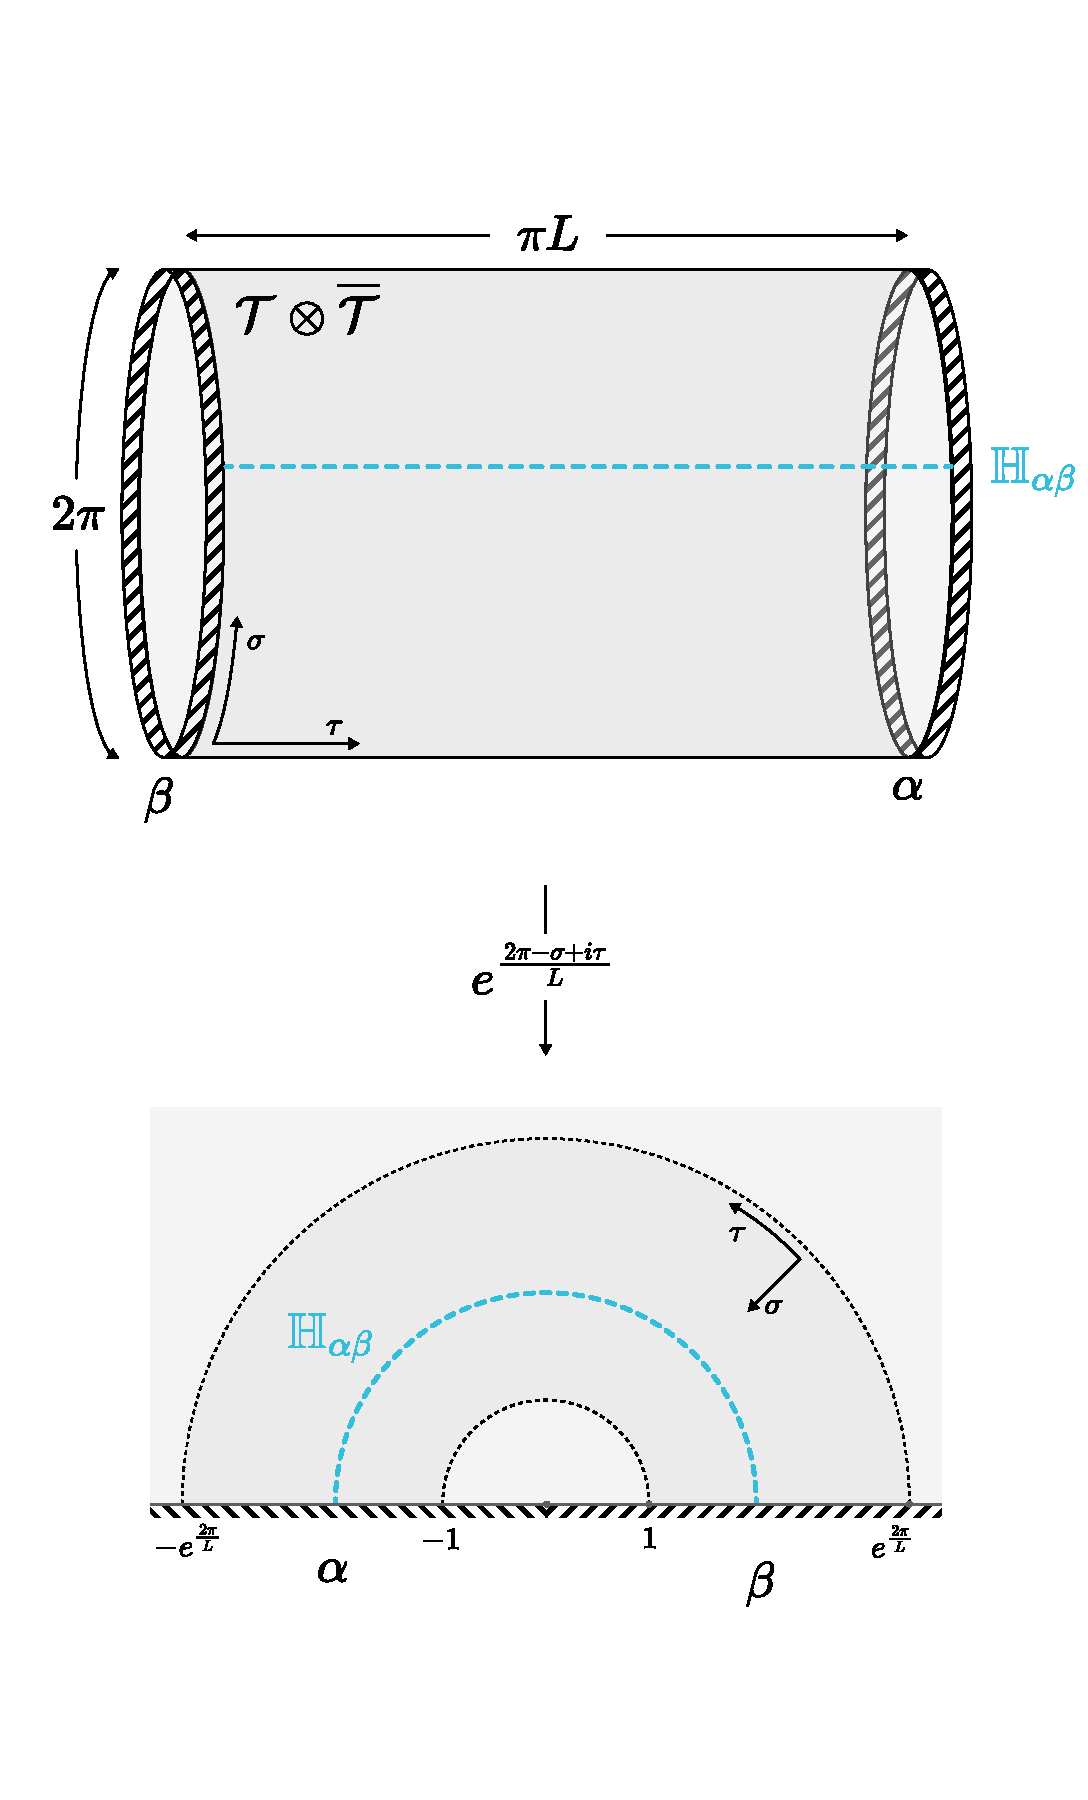
\includegraphics[width=\linewidth]{media/strip.pdf}
    \end{textblock*}
  \end{columns}
\end{frame}

\begin{frame}
  \frametitle{Cardy Trick}
  \framesubtitle{A cheeky way to generate boundaries}
  \begin{block}{Cardy's Condition}
    Matching the two conditions and expressing into characters we find that
    \begin{equation}
      S^{ji} \alpha_j \beta_j \chi_i(q) = n_{\alpha \beta}^{i} \chi_i(q)
    \end{equation}
  \end{block}
  \pause
  Which has solutions for a diagonal CFT labelled by the primaries $\alpha$
  \begin{equation}
    \alpha_j = \frac{S_{\alpha j}}{\sqrt{S_{\alpha 1}}}.
  \end{equation}
  These are also a basis of simple physical boundaries. 
\end{frame}

\begin{frame}
  \frametitle{Fusion}
  \framesubtitle{Even more boundaries!}
  If we know any topological defects, we can also fuse them with Cardy boundaries to obtain more boundaries.\par
  \begin{equation}
    \mathcal{L}\alpha = n_{\mathcal{L}\alpha}^{\beta} \beta,
  \end{equation}
  for $\beta$ simple physical boundary.
  To do this, we use modular bootstrap to come up with topological lines.
\end{frame}

\begin{frame}
  \frametitle{Gauging}
  \framesubtitle{Even even more boundaries!}
  There must be more boundaries that we can obtain through fusion.\par
  The technique is to gauge and get more Cardy boundaries.
\end{frame}

\begin{accentframe}{Generating Constraints}{Why should this be an endpoint?}
\end{accentframe}

\section{Checking Defects}
\begin{frame}
  \frametitle{g-function}
  \framesubtitle{Easy to compute \& a-theorem esque}
  \begin{figure}
    \centering
    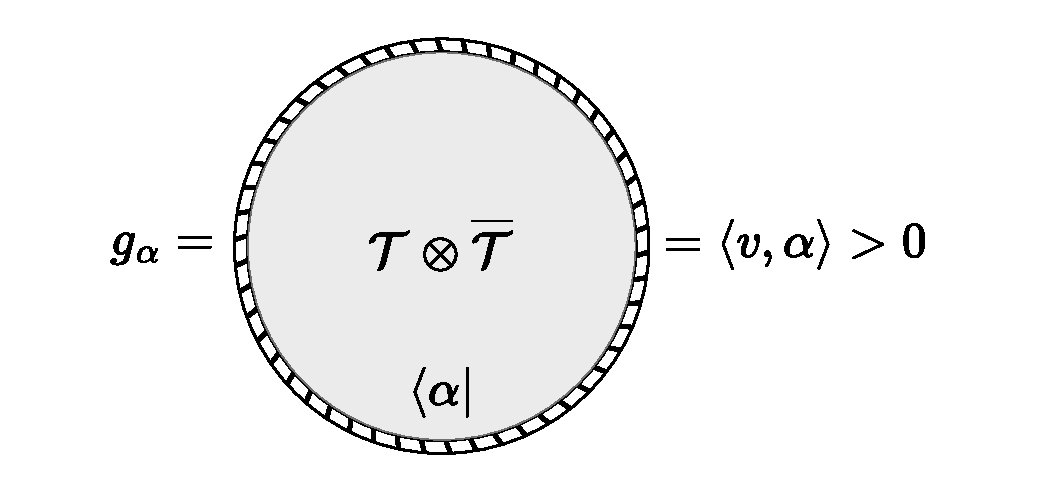
\includegraphics[width=0.5\linewidth]{media/g-function.pdf}
  \end{figure}
  is monotonically decreasing under RG. Universal as a boundary addition to the entropy. At high temperatures
  \begin{equation}
    S(\beta) = \frac{c \pi L}{6\beta} + 2\log g_\alpha + \cdots.
  \end{equation}
\end{frame}

\begin{frame}
  \frametitle{Preserved Symmetries}
  \framesubtitle{Along a flow generated by a primary}
  If a fusion symmetry commutes with a perturbation, then the symmetry is preserved along flows.
\end{frame}

\begin{frame}
  \frametitle{Preserved Symmetries}
  \framesubtitle{In the case of minimal models}
  \begin{columns}
    \begin{column}{0.55\textwidth}
      \begin{itemize}
        \item We consider perturbations of $D_{1,2}$ under $\phi_{(1,3),0}$ and $\phi_{0,(1,3)}$.
        \item Other perturbations (e.g. $\phi_{0,h}$) lead to uninteresting topological IR fixed points (since $\phi_{0,h}$ commutes with all $\bar L_n$)
        \item This preserves defects of the form $L_{(r,1)}$ which in Tricritical Ising give $\mathrm{Ising}$ fusion category.
      \end{itemize}
    \end{column}
    \begin{column}{0.45\textwidth}
    \end{column}
    \begin{textblock*}{0.40\textwidth}(0.57\textwidth+0.14\paperwidth, 0.25\paperheight)
      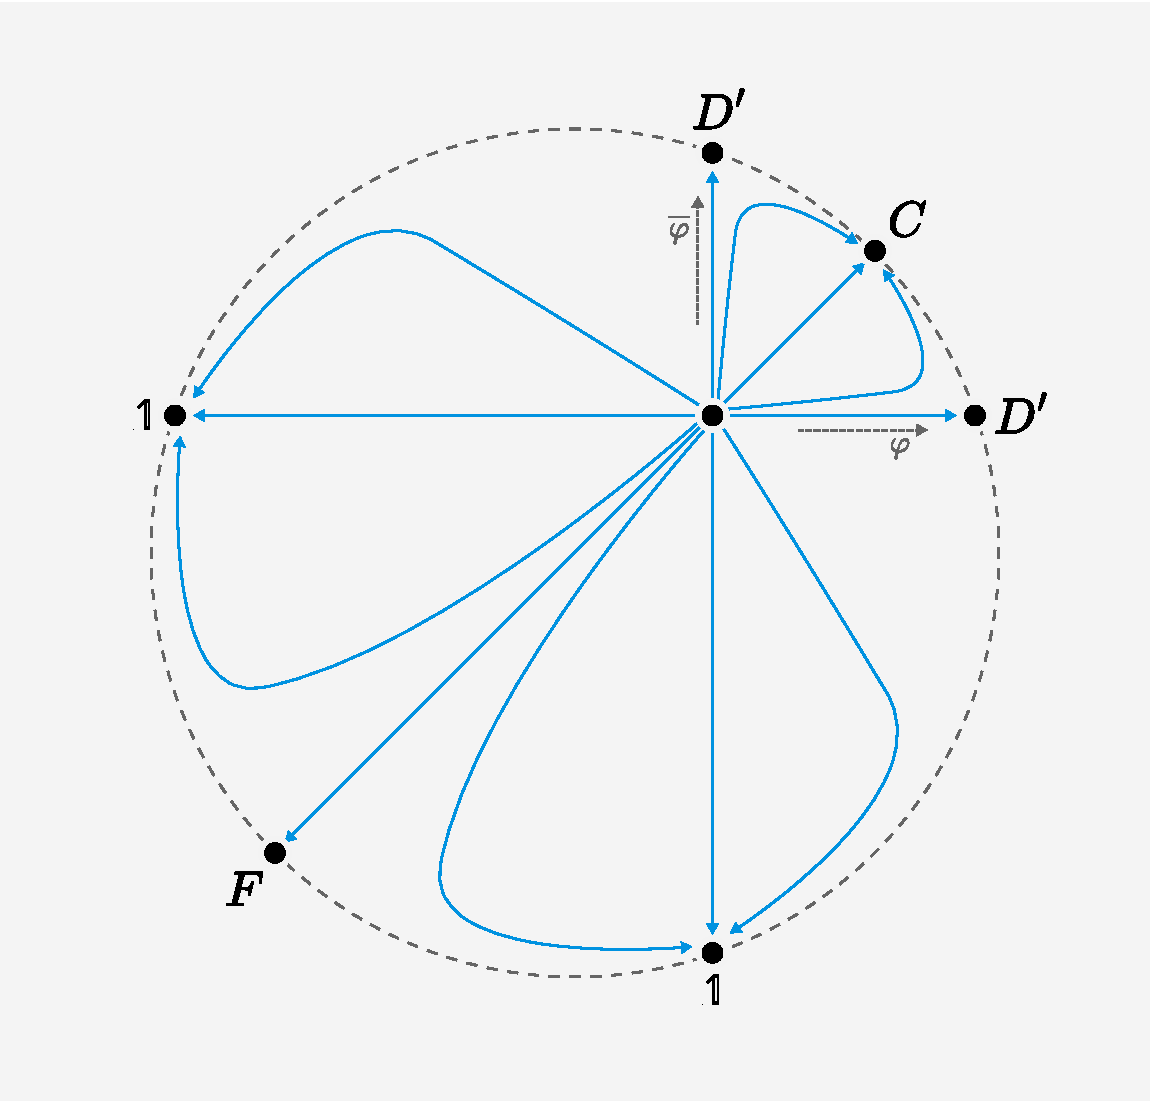
\includegraphics[width=\linewidth]{media/tricritical-flows.pdf}
    \end{textblock*}
  \end{columns}
\end{frame}


\section{Status}
\subsection{Strategy}
\begin{frame}
  \frametitle{Strategy}
  \framesubtitle{Guesses for Gaugings}
  Looking for Chiral Algebras $\mathcal{W}$
  \begin{equation}
    \mathrm{Vir} \subset \mathcal{W} \subset \mathrm{Vir}^2.
  \end{equation}
  Such that $\mathrm{TIM}^2$ is still rational. Known ones are the chiral algebras of:
  \begin{align}
    \mathcal{A} \coloneqq \frac{\mathrm{SU}(2)_8}{U(1)} && \mathcal{B} \coloneqq \frac{\mathrm{SU}(2)_2 \times \mathrm{SU}(2)_8}{\mathrm{SU}(2)_{10}} && \mathcal{C} \coloneqq \frac{\mathrm{Sp}(6)_1\times \mathrm{Sp}(6)_1}{\mathrm{Sp}(6)_2}.
  \end{align}
\end{frame}

\begin{frame}
  \frametitle{Strategy}
  \framesubtitle{Guesses for Gaugings}
  \begin{itemize}
    \item $\mathcal{A}, \mathcal{B},$ and $\mathcal{C}$ are (rational) WZW cosets related to $\mathrm{TIM}^2$ by gauging. 
    \item In subsequent gaugings we can (possibly/hopefully) find smaller algebras under which $\mathrm{TIM}^2$ is rational.
    \item Pull out Cardy boundaries and use bootstrapped TDLs to obtain more.
    \item Constrain defects based on $\mathrm{g}$-function preserved symmetry and more.
  \end{itemize}
\end{frame}

\begin{frame}
  \frametitle{Current Status}
  \framesubtitle{Progress so far}
  \begin{enumerate}
    \item Outline Numerical Results in Makabe + Watts.
    \item Describe the conjectured and numerically justified gaugings from $\mathrm{TCI}^2$ to all modular invariants of the chiral algebras of $\mathcal{A}$ and $\mathcal{B}$.
    \item Calculated Cardy states in $\mathcal{A}$ and shown that it has no defects consistent with numerical $g$ function estimation for $C$. 
    \item Bootstrapped the TDLs in $\rm{TCI}^2$ that commute with the $\mathcal{A}$, and repeating for $\mathcal{B}$.
    \item Working on identifying the smallest common chiral subalgebra in which all theories are rational.
  \end{enumerate}

\end{frame}
\subsection{Future for me}


\end{document}
